\documentclass[12pt]{report}

 % Add this line to your preamble
% Language setting
% Replace `English' with e.g. `Spanish' to change the document language
\usepackage[english]{babel}

% Set page size and margins
% Replace `letterpaper' with `a4paper' for UK/EU standard size

\usepackage[top=3cm,bottom=3cm,left=3cm,right=3cm,marginparwidth=1.75cm]{geometry}
	
% Load the setspace package
\usepackage{setspace}
\usepackage{amsmath}
\usepackage{listings}
\usepackage{xcolor}
\usepackage{multirow}
\usepackage{amssymb}
\usepackage{pgfplots}
\usepackage{float}
\usepgfplotslibrary{fillbetween}
\usetikzlibrary{arrows.meta, bending}
\pgfplotsset{compat=newest}
\usetikzlibrary{decorations.markings}
\lstdefinestyle{mystyle}{
    commentstyle=\color{gray},
    keywordstyle=\color{blue},
    numberstyle=\tiny\color{gray},
    stringstyle=\color{purple},
    basicstyle=\ttfamily\footnotesize,
    breakatwhitespace=false,         
    breaklines=true,                 
    captionpos=b,                    
    keepspaces=true,                 
    numbers=left,                    
    numbersep=5pt,                  
    showspaces=false,                
    showstringspaces=false,
    showtabs=false,                  
    tabsize=2
}

\lstset{style=mystyle}

% Useful packages
\usepackage{graphicx}
\usepackage[colorlinks=true, allcolors=black]{hyperref}
\usepackage{tikz}
\usepackage{natbib}
\pgfplotsset{width=12cm,compat=1.9}
\doublespacing

\bibliographystyle{unsrtnat}

\usetikzlibrary{shapes.arrows, positioning, arrows.meta}


\title{Theoretical framework}
\author{Riccardo Dal Cero}

\begin{document}

\maketitle

\begin{abstract}
    The main idea is to study how and whether the asymmetry of information have an impact on the cleansing effect of
    recession, replicating the model in computer  simulation.
\end{abstract}

\tableofcontents
\chapter{Introduction} 


In macroeconomic theory, the investigation of business cycles and long-term growth trajectories traditionally unfolds in
distinct academic silos, drawing a parallel to the distinct realms of quantum mechanics and Einstein's theory of
relativity in physics. This academic segregation, however, obscures a fundamental and profound question: How do business
cycles influence long-term economic growth? The exploration of this question is more than an academic exercise; it
underpins the practical understanding of short-term economic policies, such as automatic stabilizers, and their profound
long-term impacts on the economy. 

Embarking on this exploration, my research primarily dwells in the realm of theory, supplemented by rigorous simulation
and calibration exercises. The intricate complexity of business cycles, particularly evident during periods of economic
downturn and recovery, challenges empirical approaches due to the plethora of confounding variables. Thus, a theoretical
lens, rather than a purely empirical one, is employed to dissect and understand these phenomena. 

Central to this theoretical framework is an examination of the role of financial market frictions during economic
recessions. A key inquiry here is the investigation of policy interventions, such as demand stabilizers, and their
potential effect in attenuating the 'cleansing effect' of recessions. This exploration is pivotal in understanding
whether such policies might inadvertently lead to a reduced economic baseline or steady state in the long term. 
 
The conceptual foundation of this investigation is inspired by an ecological analogy the cyclical dynamics observed
between predator and prey populations in nature. This natural cycle, when observed over extended periods, reveals not
just self-contained oscillations but also underlying trends of population growth for both predators and prey. This
observation leads to a compelling analogy for economic cycles: while they appear as short-term fluctuations, they might
be underpinned by long-term growth trajectories. 

In natural ecosystems, interventions aimed at stabilizing these cycles  such as protecting prey during times of
increased predation might seem beneficial in the short term. However, such interventions often neglect the critical and
natural process of selection. This interference disrupts evolutionary mechanisms, potentially leading to unforeseen
consequences over time, such as the propagation of traits detrimental to the species' survival and adaptability in
changing environments. 

My thesis extends this analogy to the economic sphere, positing a similar selective mechanism at play in economic
systems. The primary focus is on the recession's cleansing effect, which might be analogous to natural selection in
ecology. This effect could potentially 'weed out' less productive firms, leaving a market landscape dominated by more
efficient players. The exploration aims to decipher whether such an economic 'natural selection' mechanism exists and,
if so, how it shapes the fabric of productivity, innovation, and growth in the long term. Through this lens, the
research endeavors to contribute a nuanced understanding of the intricate interplay between short-term economic
fluctuations and long-term economic evolution, offering insights into the design and implications of economic policies. 
In the following sections, we will delve deeper into specific theories that bridge the gap between business cycles and
long-term economic growth. However, it is beneficial first to embark on a brief historical journey through the evolution
of thought regarding business cycles, to understand the context and development of these interconnected economic
theories. This exploration will provide a foundation for appreciating the diversity of perspectives and the progression
of ideas that have shaped our understanding of the intricate relationship between short-term economic fluctuations and
long-term growth trajectories. 
\chapter{Literature review}
\section{Business cycle history}

\subsection{Theories Connecting Business Cycles to Long-Term Growth}

In the domain of economic theory, the relationship between business cycles (BC) and long-term growth is dissected into
two principal schools of thought. The conventional viewpoint suggests that long-term growth is chiefly propelled by
technological progress. Within this framework, technological advancements are often viewed as exogenous—arising outside
the economic model's explanatory scope, as highlighted in the seminal contributions of \cite{Sol56} and \cite{Swa56}.
This perspective treats technological progress as an independent variable that exerts influence on economic growth
without being influenced by the economy's internal dynamics. 

Contrastingly, an alternative strand of theoretical work aims to endogenize technological progress, weaving it into the
fabric of the economic process. These models embed factors such as incentives for innovation, the value of education,
and the accumulation of knowledge through economic activities, epitomizing the 'learning by doing' paradigm. A prominent
example of this approach is found in \cite{Sta90}, which posits technological progress as an emergent property of
economic behavior and incentives, rather than a mysterious external force. 

A critical aspect of the 'learning by doing' model is its premise that technological frontiers are contingent upon the
existing knowledge base, which expands primarily through practical experience. Consequently, periods of economic
expansion witness a sharp increase in the knowledge stock, driven by higher employment levels, whereas recessions tend
to stabilize or even diminish this stock due to reduced employment rates. This dynamic suggests that economies devoid of
cyclical fluctuations might attain superior steady-state growth, as employment remains consistently high, fostering
continuous technological advancement. From this perspective, the concept of a 'cleansing effect'—whereby economic
downturns eliminate low-productivity jobs and ostensibly strengthen the economy—is challenged. The elimination of even
low-productivity roles can erode the overall knowledge base. 

Such theories reframe the discourse on stabilization policies, particularly fiscal interventions, by highlighting their
role in sustaining employment and, by extension, supporting the technological frontier even in downturns. 

To illustrate this theory's implications more vividly, consider a nuanced example: an antiquated factory with limited
land resources discovers an innovative method to utilize an old tractor more efficiently. Despite the ingenuity of this
breakthrough, if the broader economy has moved beyond the technology that the tractor represents, the innovation might
not significantly contribute to the overall knowledge stock or push the technological frontier forward. This scenario
prompts a fundamental inquiry: does innovation at the lower end of the skill spectrum or within outdated technological
contexts meaningfully advance the technological frontier? Or, would it be more beneficial for economic growth to
transition such small-scale innovations into larger entities equipped with modern technologies? 

One significant critique concerns the disparity in learning opportunities across different sectors and among
individuals. The model's premise of uniform learning opportunities does not always align with the reality that some
industries, such as the technology sector, offer rapid innovation and learning environments compared to more traditional
manufacturing industries, where the pace of learning and innovation may be inherently slower due to the nature of the
work processes involved.

Furthermore, the model may not adequately address the issue of structural unemployment that can arise from technological
advancements. As certain workers benefit from "learning by doing," leading to increased productivity, others may find
their skills becoming obsolete due to automation and other technological changes. This dynamic is evident in the
automation of routine manufacturing jobs, which, while fostering "learning by doing" in fields like robotics and
software engineering, simultaneously leads to structural unemployment for workers displaced by these technologies.

Another point of contention is the potential for diminishing returns to learning. The assumption that "learning by
doing" continuously fuels growth may not hold up against the reality that initial rapid gains in productivity tend to
taper off as workers gain proficiency, suggesting that the benefits of learning may diminish over time.

The model also potentially overlooks the externalities and spillover effects associated with "learning by doing."
Technological advancements in one firm or sector do not automatically translate into broader economic growth if these
advancements remain isolated and do not benefit other sectors or industries. This is illustrated by a software company
that develops cutting-edge algorithms, enhancing its productivity but failing to contribute to the wider economy if the
knowledge remains proprietary.


This nuanced exploration challenges the simplistic notion of 'learning by doing' by questioning the value and impact of
incremental innovations within the broader economic and technological ecosystem. It underscores the complexity of
technological progress and its interplay with economic dynamics, inviting a deeper investigation into the mechanisms
that drive long-term growth and the role of policy in nurturing an environment conducive to continuous innovation and
knowledge expansion. 

The contemporary perspective on technological advancement, when viewed as a product of incremental contributions from
every market participant, appears overly simplistic. A more accurate depiction of technological progress recognizes it
as predominantly driven by those at the forefront of research. The expansion of the technology frontier is essentially
shaped by the knowledge and breakthroughs of these leading-edge innovators. Other entities in the economy adopt these
innovations at varying paces, influenced by the associated adoption costs. While firms that are not at the innovation
frontier may achieve marginal efficiency gains through adoption, the impact of such improvements is often minimal. These
marginal innovations are frequently a reflection of the adopting firms' constraints, particularly their inability to
invest in more advanced and expensive technologies. Consequently, these incremental innovations have limited potential
for widespread diffusion, as they stem from a position of necessity rather than pioneering advancement. 

Another theory describe a recession as a period in which the opportunity cost of investing in a productivity enhancing
projects is lower since the workforce is not fully in demand to produce goods. Doing this would lead in theory to higher
productivity in the period of expansion. The key role here is that the productivity-enhancing activity is costly and thus
divert capital and labor force from production as Hayek \cite{Hay33} explained. 
For this view to be valid two key aspects should be true at the same time: in the first place the
expectations about the length of the recession should reinter in the short-term otherwise it is cheaper to destroy some
production units (labor and capital) to accommodate the slow in demand. The last condition is that internal resources
must be less costly than external ones, however, it would be cheaper to higher more skilled workers and fire the low-skill
one. An additional remark is the this theory describes all those initiatives like worker formation that affect only
marginally the productivity of a firm. It misses the main mechanics in which a firm can increase its productivity sharply: thorough technical
innovation, and to do so you need a research program where the workforce is fully dedicated to it and not
diverted from production.

Another theory posits that recessions offer a period in which the opportunity cost of investing in
productivity-enhancing projects are lower, primarily because the workforce is not fully engaged in producing goods.
Theoretically, this would lead to higher productivity during subsequent periods of expansion. A crucial element in this
perspective is the acknowledgment that productivity-enhancing activities are expensive, thereby diverting capital and
labor away from immediate production, a concept Hayek \cite{Hay33} elucidated. 

For this viewpoint to hold, two critical conditions must be concurrently satisfied: firstly, expectations regarding the
duration of the recession must be short-term. If the recession is anticipated to be prolonged, it becomes economically
viable to dismantle some production units (both labor and capital) to adjust to reduced demand. Secondly, the cost of
utilizing internal resources for such productivity-enhancing ventures must be lower than the cost of acquiring external
resources. Otherwise, it might be more economical to hire more skilled workers and lay off less skilled ones.  

An additional observation about this theory is that it accounts for initiatives like worker training, which only
marginally affect a firm's productivity. This overlooks the primary mechanism through which a firm can significantly
boost its productivity: through technical innovation. To achieve substantial innovation, a dedicated research program is
essential, where the workforce is fully committed to innovation efforts rather than being diverted to current production
tasks. This highlights a gap in the theory, suggesting that while reallocating resources during recessions may offer
some productivity benefits, the most dramatic productivity improvements are likely achieved through focused
innovation and research activities, not merely through the opportunistic reallocation of resources during economic
downturns. 

An intricate theory that elaborates on the dynamics of economic recessions and the associated lower opportunity costs is
grounded in the concept of labor hoarding, as discussed in the seminal work by Clark \cite{Cla73}. This theory posits
that firms maintain employment levels higher than what immediate efficiency metrics might dictate. The rationale behind
such a strategy is to prepare for a potential surge in demand, ensuring that the firm can quickly ramp up production
without the delays associated with recruiting and training new employees. However, this strategic maneuver towards the
internal possibility frontier—where firms optimize their readiness for future demand—does not manifest as observable
changes in employment rates. Consequently, this leads to discrepancies or residuals in the statistical series of
employment, which do not align with what might be considered the level of optimal employment, a phenomenon further
analyzed in the work of \cite{BurnCrai93}. 

This labor hoarding theory offers a partial explanation for the strong pro-cyclically of measured productivity. During
economic upturns, firms can immediately respond to increased demand using their hoarded labor, thereby appearing more
productive. Conversely, during downturns, the reluctance to shed this excess labor, due to the anticipation of future
demand recovery, results in lower observable productivity levels. This behavior underscores a strategic depth in firm
management, navigating through the cyclical economic waves by balancing between immediate efficiency and long-term
responsiveness. 

Expanding on this foundation, it becomes evident that the decision to engage in productivity-enhancing activities during
recessions is not merely a reaction to lower opportunity costs but also a strategic consideration influenced by
expectations of the recession's duration and the comparative costs of internal versus external resources. If firms
anticipate a short-lived recession, the logic of hoarding labor and investing in internal productivity initiatives
becomes compelling. However, this strategy hinges on the assumption that improving the skill set of the existing
workforce or reallocating resources towards innovation is less costly than the alternative—acquiring new, possibly more
skilled labor post-recession. 

The opportunity cost (OC) approach closely aligns with the theory of labor hoarding, which seeks to elucidate the
pronounced procyclicality of measured productivity. This observation implies that during economic downturns, firms
appear to retreat towards the interior of their production possibility frontier, opting for a strategic reduction in
operational efficiency rather than workforce downsizing. This strategy is partly attributed to the invisible nature of
one crucial input—effort—to statisticians, and the economic rationale that, given the costs associated with employee
turnover, it proves more economically viable for firms to dial back effort during slumps instead of terminating
employment. 

An intriguing alternative to diminishing effort is the redirection of employee tasks from immediate production roles to
undertakings that bolster the firm's long-term productivity. At first glance, this strategy bears a resemblance to labor
hoarding but carries the added outcome that these so-called shadow activities, embraced during recessions, eventually
manifest as enhancements in total factor productivity. 

The concept of adjustment costs does not singularly confine firms from adapting their production factors according to
operational necessities. This opportunity cost mechanism could theoretically extend to a macroeconomic scale,
influencing individual entities via price adjustments. During periods marked by diminished production value, the
immediate returns from production activities (e.g., wages for workers) decline in comparison to alternative endeavors,
notably human capital accumulation, whose benefits are pegged to future earnings. This economic mechanism could
precipitate a resource reallocation towards these alternative activities. The empirical observation that education
durations tend to extend during economic recessions lends credence to this argument. Nevertheless, with the exception of
leisure, most sectors shadow the movements of aggregate GDP. Thus, if productivity-enhancing activities (PEAs) are to
occur during recessions, the resource reallocation process must predominantly unfold within the firms themselves. 

One notable deviation might be labor reallocation. As demonstrated by \cite{DavHalt92}, job destruction exhibits a
more countercyclical pattern compared to job creation. Viewing job reallocation through the lens of both destruction and
creation suggests a countercyclical trend, positing job reallocation as an investment in cultivating superior
firm-worker matches, thereby sowing the seeds for heightened productivity in the future. \cite{DavHalt92}further
postulate, within the framework of a model featuring a representative agent, that economic recessions present an optimal
window for labor reallocation, highlighting a strategic dimension to workforce management during downturns that might
ultimately contribute to long-term productivity gains. 
 
The "lame ducks" theory, initially proposed by \cite{CabHarm94}, offers an intriguing perspective on
recessions as mechanisms that phase out less profitable, outdated capital. This theory delineates how the destruction of
older units during downturns is more pronounced than the construction of new ones, characterizing recessions as periods
marked by the systematic elimination of obsolete capital, hence the moniker "lame ducks" theory. Notably, this framework
sheds light on observations documented by \cite{DavHalt92}, positioning it as a prominent theoretical
approach that will be delved into more thoroughly in subsequent discussions. 

Despite its insights, this model lacks consideration of the financial dimensions of firms, an aspect addressed by the
theoretical work of \cite{OsePap17}. Their research weaves the financial decision-making process into the
broader context of intertemporal capital decisions, highlighting how financial frictions influence the lender's
participation constraint. The study reveals that, despite financial frictions, the cleansing effect of recessions on
productivity persists, potentially leading to a more pronounced productivity surge during expansion phases. This
analysis serves as a pivotal foundation for the new theoretical framework introduced in this thesis, marking a
significant departure from traditional views and emphasizing the multifaceted impact of recessions on firm productivity
and economic recovery. 

In the forthcoming sections, / we will explore the
theoretical underpinnings that form the basis of the new, streamlined theoretical framework introduced in this thesis.
Our examination begins with the insights of \cite{CabHarm94}, focusing on the interplay between the
destruction and creation margins in economic cycles. Subsequently, we will delve into the work of \cite{OsePap17}
(2017), which sheds light on the financial dimensions, particularly how capital lending frictions can precipitate
misallocations. These studies collectively inform the development of our theoretical framework, setting the stage for a
comprehensive analysis of economic dynamics and firm behavior during recessions. 

\section{Literature review of theoretical models}
\subsection{Introduction}
This section of the literature review examines two influential theoretical models that analyze the cleansing effect of
recessions on the economy. The first model, introduced by \cite{CabHarm94}, utilizes a vintage model of
creative destruction to investigate how industries adapt to cyclical demand variations. This model is pioneering in its
approach, highlighting how recessions can facilitate the removal of outdated and less efficient production units,
potentially leading to an overall increase in industry productivity. The model's insights are derived from a framework
where production units of varying vintages coexist, and the rate of technological adoption plays a crucial role in
determining industry responses to economic fluctuations.

In contrast, the second model explored in this review, by \cite{OsePap17}, introduces financial frictions into
the analysis of the cleansing effect of recessions. This addition brings a new layer of complexity to the understanding
of how economic downturns affect firm dynamics, particularly by influencing the selection process through which firms
enter and exit the market. The model underscores the role of credit constraints in mediating the impact of recessions,
suggesting that financial frictions can dampen the potential productivity gains that might otherwise arise from the
purging effects of a downturn.

Both models rely on numerical methods to solve their respective frameworks, acknowledging the intricate dynamics and
non-linearities inherent in their analyses. By comparing these models, this review seeks to illuminate the diverse
mechanisms through which recessions can influence economic outcomes, as well as the varying implications of introducing
different types of market frictions into theoretical frameworks.
\subsection{The cleansing effect by Caballero}

In the first paper that rationalizes the cleansing effect of recessions, \cite{CabHarm94} and published in the American
Economic Review in 1994, the primary aim was to investigate how
industries respond to cyclical variations in demand. They did this by employing a vintage model of creative destruction.
The underlying concept postulates that the processes of creation and destruction within an industry partially explain
business cycles. Industries continuously experiencing creative destruction can adapt to demand fluctuations in two
ways: by adjusting the rate at which they produce new units embodying advanced techniques or by altering the
rate at which outdated units are retired. The model they used incorporated heterogeneous firms, where production units
embodied the most advanced technology at the time of their creation. The costs associated with creating new units
slowed down technology adoption, resulting in the coexistence of production units with varying vintages.
\par
Key to understanding how firms adapt to business cycles are the concepts of the creative margin and the destruction
margin. For example, a reduction in demand can be accommodated either by reducing the rate of technology adoption or by
retiring older production units. One of the primary factors determining which margin is more responsive to business
cycles is the adjustment cost. When this cost follows a linear pattern, the study shows that insulation is complete, and
the industry's response relies exclusively on its creation margin. Consequently, the creation margin becomes smoother
over time in comparison to the destruction margin, which exhibits greater responsiveness to the business cycle.
\par
Crucially, Caballero and Hammour's research \cite{BlaDia90} offers theoretical insights supported by empirical
evidence. Their findings on the cyclical nature of the destruction margin align with the studies conducted by Blanchard
and Diamond \cite{BlaDia90}, as well as Steven Davis and John Haltiwanger \cite{DavHalt92}, in their respective works
from 1990. This
convergence between theoretical framework and empirical substantiation underscores the importance of comprehending the
dynamic interplay between creative destruction and business cycles, which significantly influences how industries
respond to economic fluctuations.
\par
In their study \cite{DavHalt92}, where they assess the heterogeneity of employment changes at the establishment level in
the U.S. manufacturing sector from 1972 to 1986, it is revealed that job destruction exhibits procyclical tendencies,
responding more robustly to downturns in the economic cycle compared to the creation rate, in line with the theoretical
model proposed by Caballero and Hammour \cite{CabHarm94}. The authors leverage a natural experiment inherent in the data
to examine whether the structure of adjustment costs can account for the behavior of these two margins. This natural
experiment arises from the asymmetric nature of business cycles, with recessions being shorter but more severe than
expansions. The theoretical model predicts that these differences should be attenuated in the creation process, a
prediction that is substantiated by the data since creation exhibits relative symmetry around its mean, while
destruction displays a high degree of asymmetry.
The underlying concept driving the behavior of the destruction margin can be traced back to the theories of Schumpeter
and Hayek.  They suggest that recessions represent periods during which unprofitable or outdated techniques are pruned
from the economy, leaving behind the most efficient firms \citet{HaCa07}.
\subsubsection{Theoretical model}
The model in question is a vintage model that simulates an industry experiencing exogenous technological progress.
Within this model, production units are constructed using a fixed proportion of labor and capital, and they are
continually being created and phased out. Notice that only the creation of new production units
incurs a cost. This simplification is plausible, particularly in the context of the United States, where the expense
associated with hiring is typically higher than the cost of termination, as demonstrated by Abdulkadiroğlu and Kranton
(2003) \cite{AbdKra03}. 
\par
In this model, when a production unit is created at a specific time \(t_0\), it embodies the most advanced technology
available at that moment and consistently generates a uniform output represented by \(A(t_0)\) throughout its
operational lifetime. The productivity of this technology denoted as \(A(t)\), experiences continuous growth at an
exogenously determined constant rate \(\delta \ge 0 \). This growth in technology can be interpreted in two ways: either
as the adoption of new technology or as a product innovation. In the latter scenario, a continuum of perfectly
substitutable products can yield varying levels of output.

\[\left[ f(a,t) \qquad 0\leq a \leq \overline{a}(t) \right]\]

The above function represents the cross-sectional density of the production units aged \(a\) at time \(t\), where
\(\overline{a}(t)\) is the age of the oldest production unit at time \(t\). The first assumption is that \(f(a,t)\) and
\(\overline{a}(t)\) are continuous functions. The mass of production units at time \(t\) is given by:

\[N(t) = \int_{\overline{a}(t)}^{0}f(a,t)da\]

\(N(t)\) is a measure of either the industry's capital stock or its employment, due to a fixed share of capital and
labor. Thus, the industry's output is given by:

\[Q(t) = \int_{\overline{a}(t)}^{0}A(t-a)f(a,t)da\]

The deterioration of production units involves both an exogenous depreciation rate \(\delta\) and an endogenous
destruction process, which impacts \(f(a,t)\) at its limits. The count of production units surviving for \(a\) years is
expressed as: 

\[f(a,t)= f(0,t-a)e^{-\delta a} \quad \text{where } 0 < a \leq \overline{a}(t)\]

The production flow is determined by:

\[\dot{N}(t) = f(0,t) [1-\overline{\dot{a}}(t)] + \delta N(t)\]

Here, the first term represents the production rate, while the second term encapsulates the destruction rate,
encompassing the obsolescence rate \(f(\overline{a})(t)\), the technological obsolescence change over time
\(-f(\overline{a})(t)\overline{\dot{a}}(t)\), and the depreciation rate \(\delta N(t)\). 

The assumptions made by the authors are denoted as \(\forall t \mid f(0,t)>0 \cup  \overline{\dot{a}}(t)<\).

The alteration in output concerning these flows is articulated as:

\[\dot{Q}(t) = A(t)f(0,t) - A(t-\overline{a}(t))f(\overline{a}(t),t) \cdot [1-\overline{\dot{a}}(t)] + \delta Q(t)\]

The authors define a perfectly competitive industry in partial equilibrium, where supply is dictated by free entry and
perfect equilibrium. Additionally, they introduce a cost function related to creating new production units: 

\[c = c\left(f\left(f(0,t)\right)\right) \quad \text{where } c(\cdot)>0, \, c'(\cdot)\leq 0\]

This cost function is contingent on the creation rate, implying that higher creation rates correspond to increased
costs. The equilibrium condition is established by equating the cost of unit creation to the present discounted value of
profits throughout its lifespan. The authors set the cost of a production unit to 1, and \(P(t)\) is the price of a unit
of output. Thus, the profits generated at time \(t\) by a production unit aged \(a\) are defined as: 

\[\pi(a,t)= P(t)A(t-a)-1\]
\[\overline{a}[t+T(t)] = T(t)\]

Here, \(T(t)\) signifies the maximum lifetime of a unit created at \(t\). At any given time \(t\), the free entry
condition is expressed as: 

\[ c(f(0,t)) = \int_{t+T(t)}^{t}\pi(s-t,t)e^{-(r+\delta)(s-t)\,ds} \]

In the above equation, where \(r>0\) represents the exogenously determined instantaneous interest rate, the determination of
the exit of a production unit is contingent upon continuous \(P(t)\) and the instance when the profits generated by a
unit being destroyed reaches zero. This occurrence signifies the moment when the oldest unit operational at time \(t\),
denoted as \(\overline{a(t)}\), must adhere to the equation: 

\[P(t)A(t-\overline{a}(t))=1\]

The authors posit that \(P(t)\) exhibits a decreasing trend due to the model's assumption regarding endogenous
destruction, specifically \(\overline{\dot{a}(t)}<1\). To see, differentiate 
\[\dot{P}(t)=-\gamma\left[1-\overline{\dot{a}}P(t)\right]\]
Consequently, when the profits of a production unit diminish to
zero for the first time, it will be subject to destruction. 

On the demand side, the authors assume a unit-elastic demand function and consider the aggregate expenditure as
exogenous 
\(\overline{D}(t)=P(t)Q(t)\). 
The equilibrium is a path \(\left\{f(0,t),\overline{a}(t),T(t),Q(t)\right\}_{t \geq 0}\) that satisfy the following
conditions:
\begin{enumerate}
    \item \label{eq_2.1} 
        \begin{align*}
            Q(t) &= \int_{\overline{a}(t)}^{0}A(t-a)f(a,t)da
        \end{align*}
    \item \label{eq_2.2}
        \begin{align*}
            f(a,t)&=f(0,t-a)e^{-\delta a}      
        \end{align*}
    \item \label{eq_2.3}
        \begin{align*}
            T(t)&=\overline{a}\left(t+T(t)\right)        
        \end{align*}
    \item \label{eq_2.4}
        \begin{align*}
            c(f(0,t))&=\int_{t}^{t+T(t)}\left[P(s)A(t)-1\right]e^{-(r+\delta)(s-t)}\,ds
        \end{align*}
    \item \label{eq_2.5}
        \begin{align*}
            P(t)A(t-\overline{a}(t))&=1
        \end{align*}
    \item \label{eq_2.6}
        \begin{align*}
            P(t)Q(t)&=\overline{D}(t)
        \end{align*}
\end{enumerate}

The first three equations (\ref{eq_2.1}, \ref{eq_2.2}, \ref{eq_2.3}) and the fifth one (\ref{eq_2.5}) suffice to
delineate the trajectories of \(T(t)\), \(P(t)\), and \(Q(t)\), which are determined by \(\left\{f(0,t),
\overline{a}(t)\right\}\). To affirm the robustness of the conditions expressed in equations \ref{eq_2.6} and
\ref{eq_2.5}, it is possible to derive these equations as first-order conditions for the maximization of a number of
perfectly competitive firms holding production units. 

To comprehend the functioning of endogenous destruction, let's consider a scenario with constant demand. In this case,
both the destruction and creation rates change only due to supply factors. This steady state is characterized by a
constant lifetime of production units \(T(t) = \overline{a}(t) = \overline{a}^*\), resulting in a time-invariant age
distribution \(f(a,t) = f^*(a)\). Equation \ref{eq_2.5} implies that the price \(P(t)\) must consistently decrease at a
rate \(\sigma\). Higher innovation rates lead to increased productivity, raising the supply and consequently lowering
the price. Equation \ref{eq_2.2} reveals that the distribution of production units in the steady state follows a
truncated exponential distribution: 

\[f^*(a) = f^*(0)e^{-\delta a} \quad 0 \leq a \leq \overline{a}^*\]

Using free entry conditions (\ref{eq_2.4}) and the clearing condition (\ref{eq_2.6}), one can determine the creation and
destruction ages \(f^*(0)\) and \(\overline{a}^*\). Equations \ref{eq_2.1} and \ref{eq_2.5} yield the cost function and
productivity of a new production unit: 

\[\label{eq_2.7} c(f^*(0)) = \frac{e^{\gamma \overline{a}^*} - e^{-(r + \delta)\overline{a}^*}}{\gamma + r + \sigma} - \frac{1 - e^{-(r + \delta)\overline{a}^*}}{r + \delta}\]

\[\label{eq_2.8} f(0) = \frac{(\sigma + \delta)\overline{D}^*}{e^{\sigma \overline{a}^* - e^{\delta \overline{a}^*}}}\]

The authors then normalize the creation rate:

\[N = f^*(0) \cdot (1 - e^{\delta \overline{a}^*})\]

In the steady state, this is given by:

\[(9) \label{eq2.9}CC^* = \frac{\delta}{1 - e^{-\delta \overline{a}^*}}\]

Considering a special case where the creation cost is a constant \(c\), i.e., \(c(f^*(0)) = c\), substituting into
equation \ref{eq_2.7} allows retrieval of \(\overline{a}^*\). The effect of technological rate \(\sigma\) on
\(\overline{a}^*\) is decreasing, as a higher innovation rate increases the opportunity cost of delayed renovation,
while a higher cost of creating new units lowers the renovation rate. An optimal lifetime of production units increases
with higher \(r\) and \(\delta\) as it becomes harder to recover creation costs. 

Now, dropping the assumption of constant demand, we examine how the industry adjusts to demand fluctuations. Two ways
are identified in which the industry adapts production to meet demand: by reducing the rate of creation \(f(0,t)\) and
by increasing the rate of endogenous destruction \(f(\overline{a}(t),t) \cdot [1-\overline{\dot{a}}(t)]\), thus reducing
\(\overline{a}\), the age at which units are demolished. 

These two adjustments interact, leading to a reduction in demand causing the most outdated units to be scrapped,
rendering them unprofitable. However, if the recession is partially accommodated by a reduction in the creation rate,
the effect on the destruction margin is diminished. The authors argue that the extent to which creation will "insulate"
existing units from variations in demand depends on the marginal cost of creating new units \(c'f(0,t)\). When the
marginal cost of creation is zero, demand fluctuations are entirely adjusted by the creation margin. This is exemplified
in the case where \(c(f(0,t)) = c\). In such instances, the insulation effect is complete, as there is no need to retire
older units. Lowering \(f(0,t)\) is sufficient, and it is cheaper than reducing the life of existing production units. 

The insulation effect is not solely due to asymmetric adjustment costs on the creation and destruction margins. Complete
insulation would occur even with linear adjusting costs. The creation rate in the case of constant creation cost is
given by: 

\[\label{eq_2.10} f(0, t) = \frac{\dot{\bar{D}}(t) + \delta \bar{D}(t) + P(t) A(t - \bar{a}(t)) f(\bar{a}(t), t)[1 -
\dot{\bar{a}}(t)] - \dot{P}(t) Q(t)}{P(t) A(t)}\] 

In the attained equilibrium, variations in demand are entirely offset by adjustments at the creation margin denoted as
\(f(0, t)\), with \(\overline{a}(t)\) remaining steady at the destruction margin. The creation process effectively
counteracts the impact of demand fluctuations on the price \(P(t)\), effectively shielding existing units from demand
changes. The price \(P(t)\) experiences a constant decline at a rate represented by \(\sigma\), reflecting the pace of
technical progress. This consistent decline in \(P(t)\) serves as a clear signal for production units to function
optimally throughout their constant lifetime \(\overline{a}(t)^*\). \\
In the aforementioned scenario, the destruction rate is not constant, but it does not respond to demand through
variations in the age \(\overline{a}(t)^*\) at which units are destroyed. Instead, variations in the creation rates have
an impact on the number of units that reach obsolescence. If fewer units are created, fewer units become obsolete after
\(\overline{a}(t)^*\) periods. It is noteworthy that any modification leaving equations \ref{eq_2.3} to \ref{eq_2.5}
independent of \(\overline{D}(t)\) and \(f(0,t)\) does not alter the full-insulation results. 
\\
Interestingly, assumptions such as perfect competition, industry-wide return to scale, and perfect foresight are not
necessary for these conclusions. The latter is particularly noteworthy as it asserts that fully accommodating demand on
the creation side only requires knowledge of current conditions. As long as the non-negativity constraint on \(f(0,t)\)
is never binding, implementing equilibrium behaviors does not necessitate expectations of future demand. 
\subsubsection{Application of the model}
The model undergoes calibration utilizing Job-flow data and Industry production data. The former facilitates the
replication of job creation dynamics, while the latter is employed to mimic the behaviors of firm creation and
destruction in the manufacturing industry. To capture these dynamics, the marginal cost of creating new production units
is stipulated as positive \(c'f(0,t)\). This allows for a partial insulation effect, and the destruction margin responds
to demand fluctuations. However, introducing a dependency of \(c\) on \(f(0,t)\) compromises the analytical tractability
of the system (Equations \ref{eq_2.1} - \ref{eq_2.6}). Consequently, the authors resort to methods such as multiple
shooting to ascertain the optimal equilibrium and subsequently employ an iterative procedure to converge to the correct
expected creation rate. 

For numerical solutions, the authors adopt a linear formulation:

\[c(f(0,t))=c_0+c_1f(0,t)\]

To gain a deeper understanding of how creation and destruction respond to demand, the authors simulate sinusoidal demand
using the equation: 

\[\overline{D}(t)=1+0.07\sin(t)\]

The results are visualized in the image below, depicting the feedback of normalized creation and destruction (CC and DD)
to changes in demand. 

\begin{figure}
    \centering
    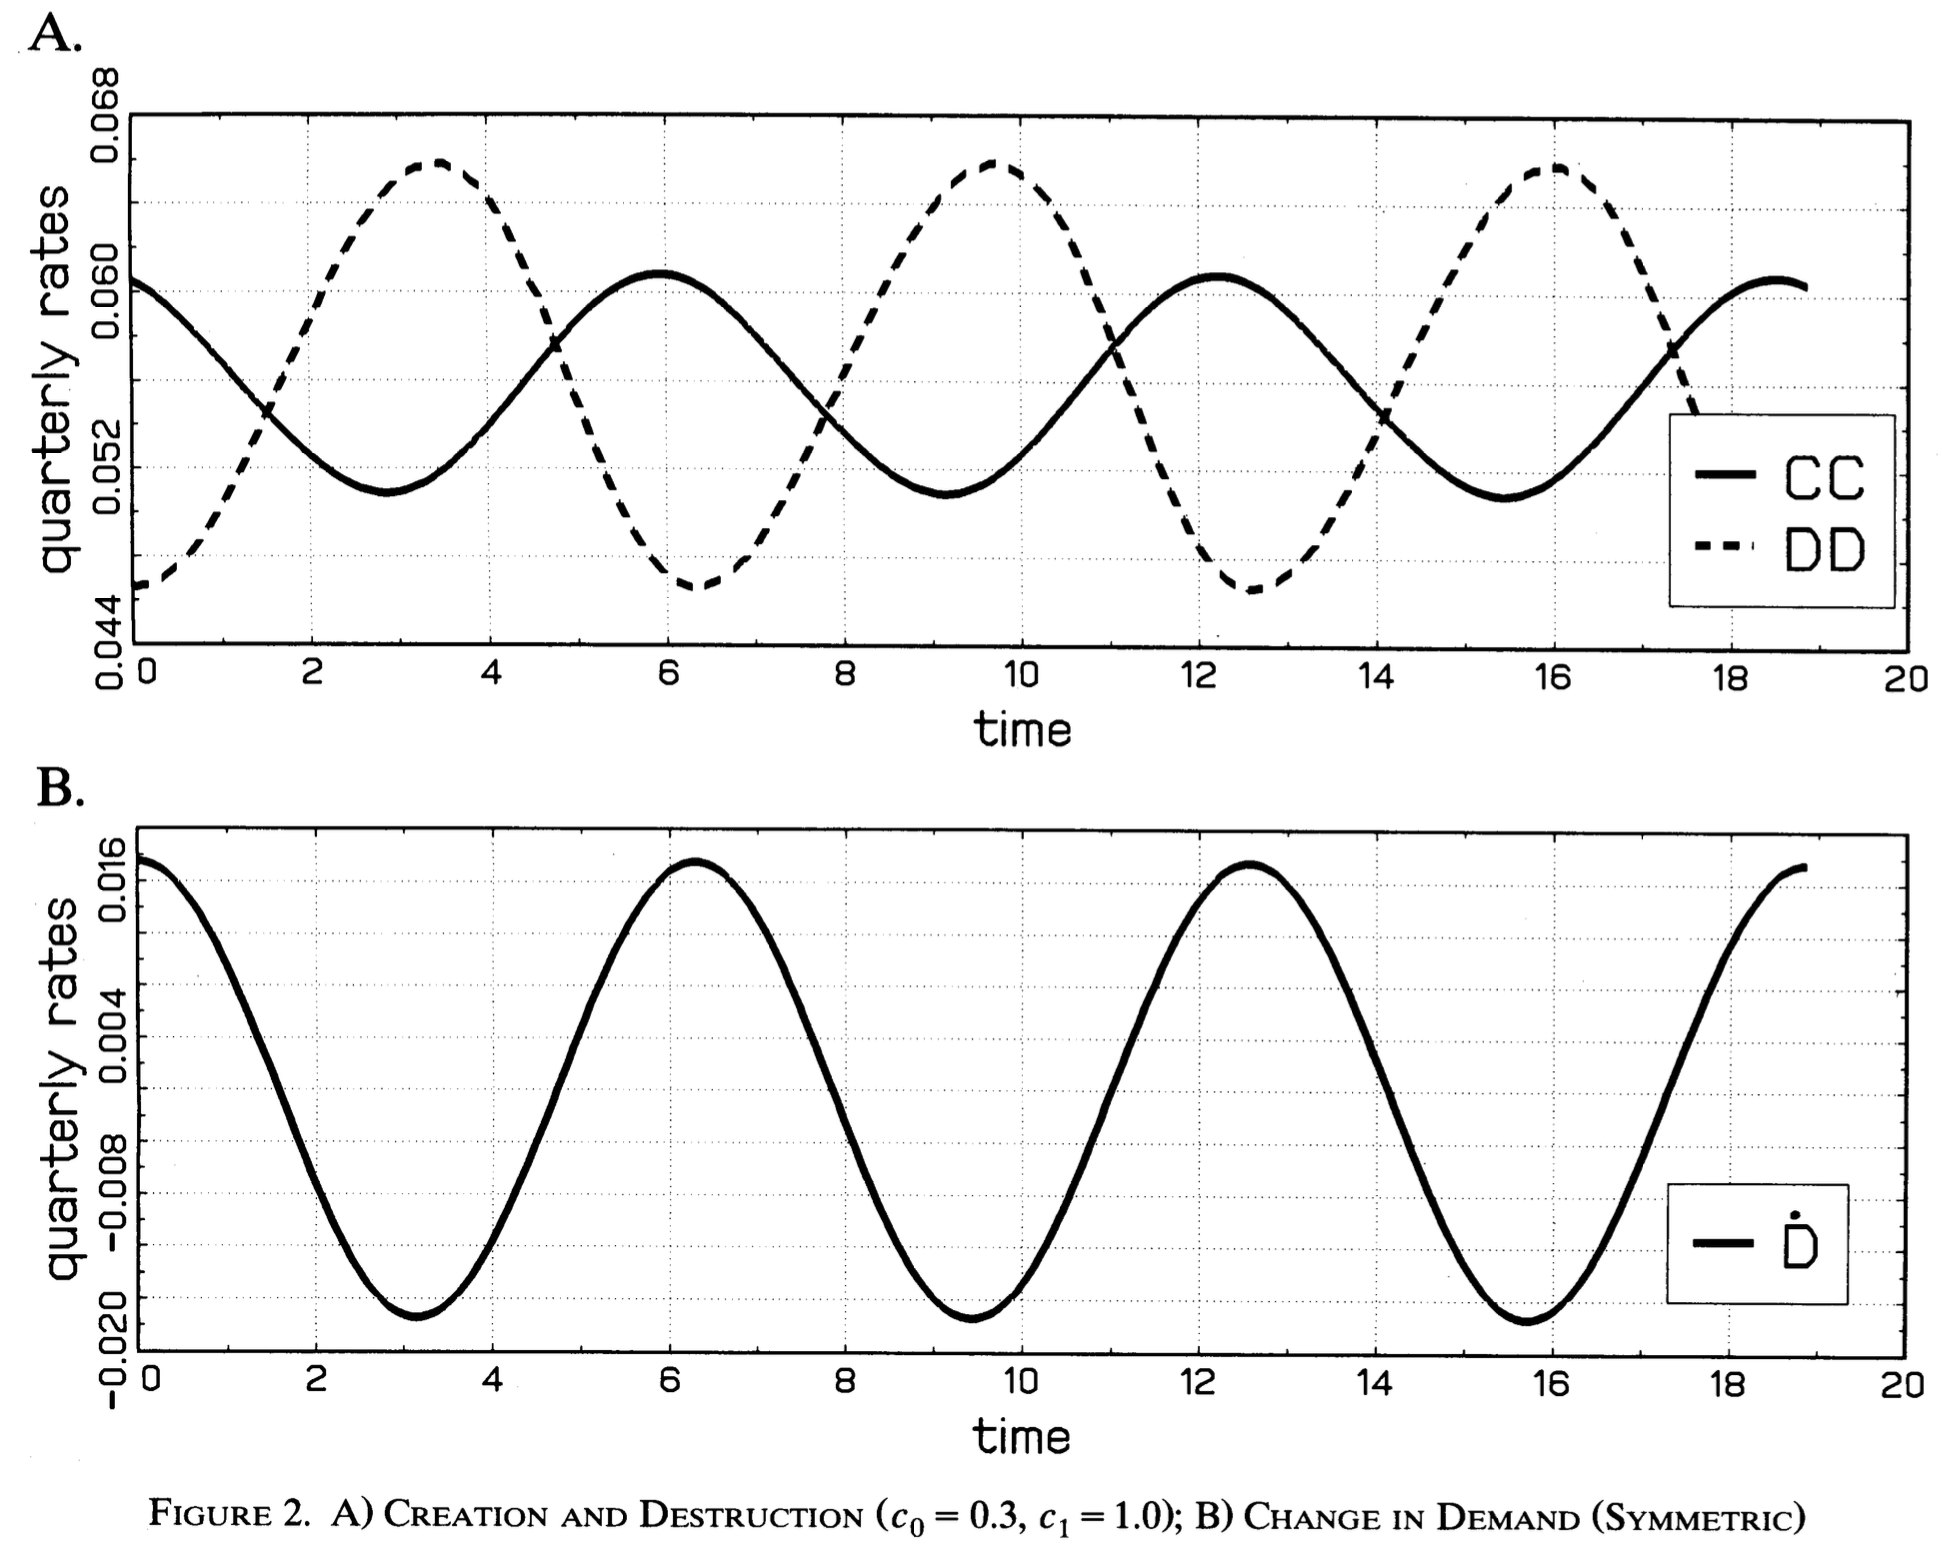
\includegraphics[scale = 0.4]{figure/Plot2.1.png}
    \caption{Figure 1. A Creation and destruction \(c_0=0.3, c_1=1\) B Change in demand (Symmetric)}
    \label{plot:2.1}
\end{figure}

The plot clearly illustrates that the insulation effect is only partial; otherwise, DD would have remained flat, as in
the case with \(c(f(0,t)=c)\). From a mathematical perspective, destruction responds to demand as equations
\ref{eq_2.3}-\ref{eq_2.5} are no longer independent of the path \(f(0,t)\) and demand. From an economic standpoint,
increasing creation costs smoothen the creation process. In scenarios with a nearly flat innovation rate, firms during
crises cannot fully accommodate lower demand, nullifying the adoption of new production units, as the marginal costs
would exceed the reduction in existing production units. \par
In the considered model, production units integrate labor and capital in fixed proportions to generate output. Each unit
can be conceptualized as contributing to job creation within the industry, and job-flow data serves as a metric for
quantifying the flows of production units. 

Datasets that closely align with the theoretical CC and DD series have been compiled by 
\cite{DAvHalt90,DavHalt92} and  \cite{BlaDia90}, drawing from various sources. The primary focus
lies on the dataset curated by Davis and Haltiwanger, who leverage the Longitudinal Research Database to construct
quarterly series for U.S. manufacturing plants spanning the period 1972:2-1986:4. 

In their empirical approach, \cite{DavHal94}utilize output to empirically determine demand, employing the growth
rate of the industrial production index as a proxy for output growth. Notably, in the foundational theoretical model,
\(Q(r)\) is smoothed by price movement, with the elasticity of demand determining the extent of smoothing, assumed to be
equal to 1. While the theoretical model maintains a constant dividend wage, the authors acknowledge that considering
a procyclical dividend wage, as in the case of general equilibrium with correlated industry shocks, may dampen the
effect of demand shocks. However, they assert that this adjustment would alter only the magnitude, not the direction, of
the analysis. 

The figure below illustrates the data that the model seeks to replicate, showcasing job creation, job destruction, and growth.

\begin{figure}
    \centering
    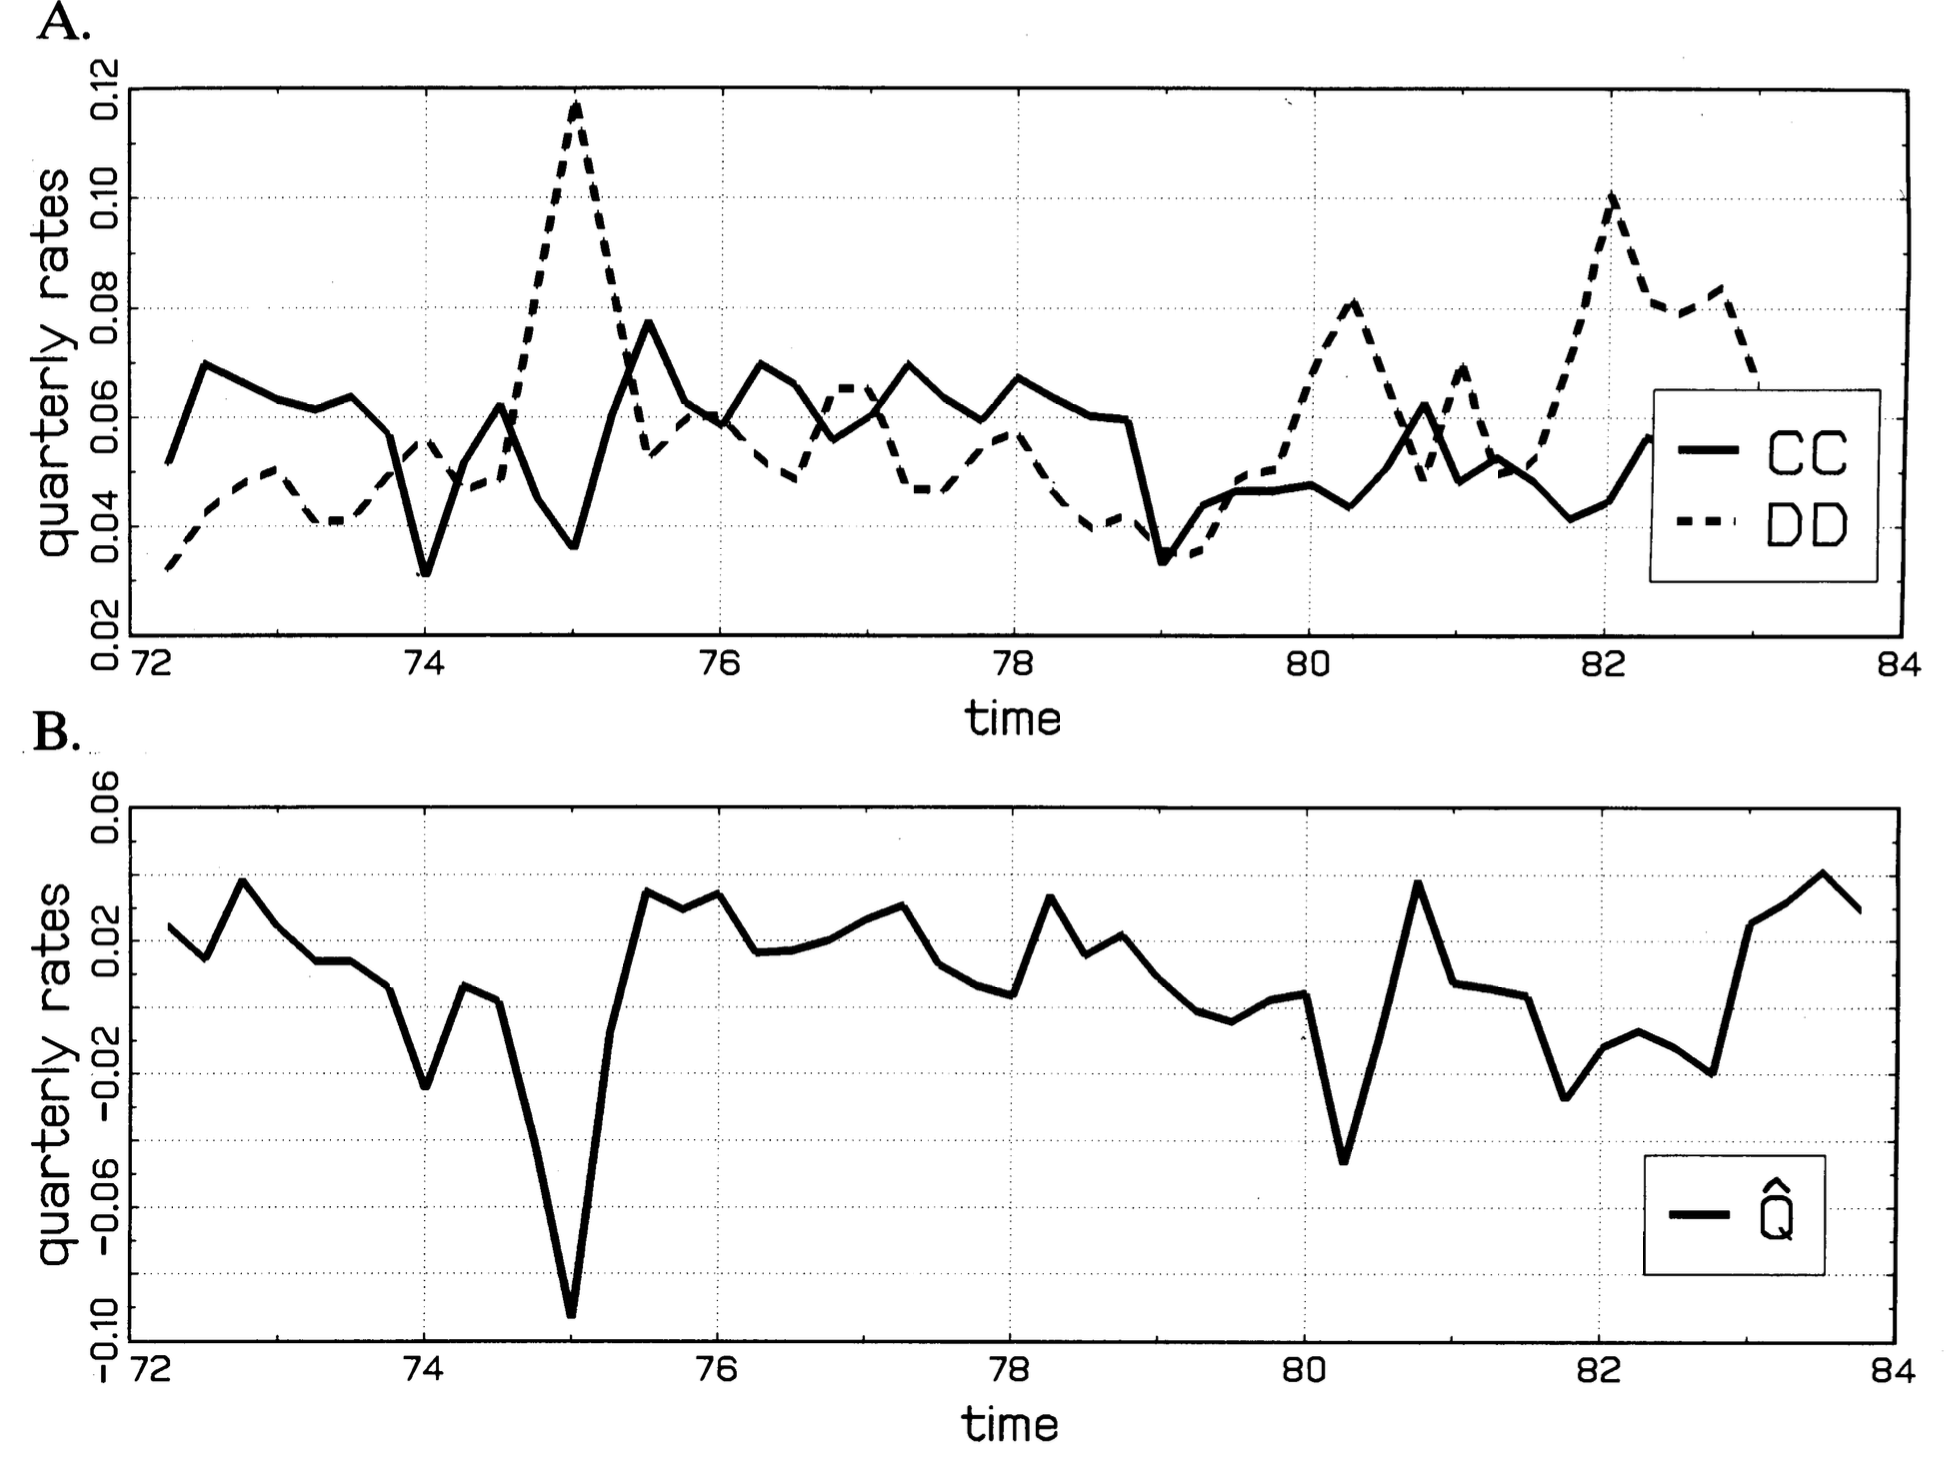
\includegraphics[scale = 0.4]{figure/Plot2.2.png}
    \caption{Figure 1. Job creation and job destruction in U.S. Manufacturing B Index of the industrial production}
    \label{plot:2.2}
\end{figure}

To discern the characteristics of the series, the authors perform regression analysis on sectoral rates of job creation
and job destruction against leads and lags of the corresponding rates of growth. They find that job creation is less
responsive to demand fluctuations, while job destruction exhibits a more countercyclical behavior. 
\begin{figure}
    \centering
    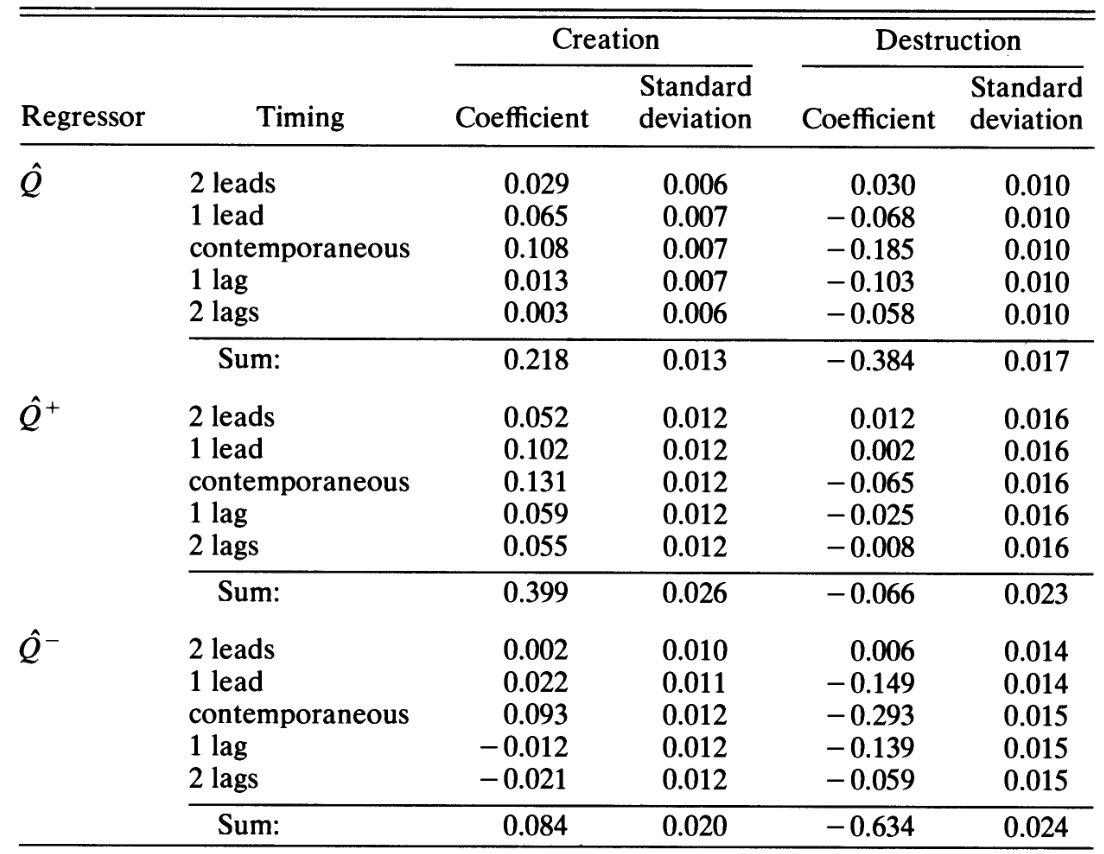
\includegraphics[scale = 0.4]{figure/Plot2.3.png}
    \caption{Table 2.1. Job Creation and Job Destruction in U.S. Manufacturing Response to Output Growth}
    \label{Table 2.1.}
    \footnotesize textit{Notes}: The table presents the reaction of job creation to the growth rate of the industrial
    production index. The latter is categorized into values above and below its mean (Q). The table encompasses
    quarterly observations for the two-digit SIC industries during the period 1972:2-1986:4. The coefficients are
    uniformly constrained to be equal across all sectors, with the exception of a constant (not shown).  
\end{figure}
The initial finding indicates that the rate of job destruction displays greater responsiveness to changes in sectoral
activity compared to the rate of job creation. Specifically, the sums of coefficients are -0.384 for job destruction and
0.218 for job creation showed in the table \ref{Table 2.1.}, the same results as in \cite{DAvHalt90,DavHalt92} and in
\cite{BlaDia90}.
The authors capitalize on a natural experiment rooted in the intrinsic asymmetric characteristics of business cycles.
Recessions, marked by brevity but intense contractions, provide the backdrop for the authors' model. This model
endeavors to emulate the creation rate while concurrently mitigating the impact of asymmetric cyclicality inherent in
business cycles. The empirical evidence supporting this model's behavior is encapsulated in Table \ref{Table 2.1.},
wherein two distinct scenarios are explored: output growth trajectories above \(Q^+\) and below \(Q^-\), relative to
their respective means. The table meticulously delineates how creation and destruction rates respond to these deviations
in output growth. 
\par
The salient observation emerges regarding creation rates, elucidating that they exhibit a more rapid and robust response
in instances of vigorous output growth, as opposed to scenarios where the output growth rate experiences a reduction. On
a contrasting note, the destruction margin, in line with the model's projections, manifests heightened sensitivity to a
decline in output. This responsiveness is particularly pronounced from one quarter before the onset of the shock to one
quarter after. Notably, during expansionary phases, the mean response of the destruction margin is -0.066, a notably
milder reaction compared to the recessionary case where the mean response stands at -0.634. 
\par
These empirical outcomes seamlessly align with the predictions of the model. Specifically, the creation rate exhibits
heightened responsiveness during expansionary phases, given their cyclical and symmetric nature. In contrast, the
asymmetric and non-cyclical nature of recessions triggers a more substantial decline in the production unit rate, in
line with the model's expectations. 
\par 
In order to better understand the asymmetrical behavior the authors simulate an asymmetrical demand function:
\[\cdot{\overline{D}}(t)=0.05[\cos(t)+\sin(t)] - 0.016 \sin(2t)-0.003\cos(3t)\]
\[\overline{D}(t)=1\quad r = 0.065, \delta =0.15, \gamma=0.028, c_0=0.3, c_1=1.0\] 
The results are depicted in \ref{plot:2.4}
\begin{figure}
    \centering
    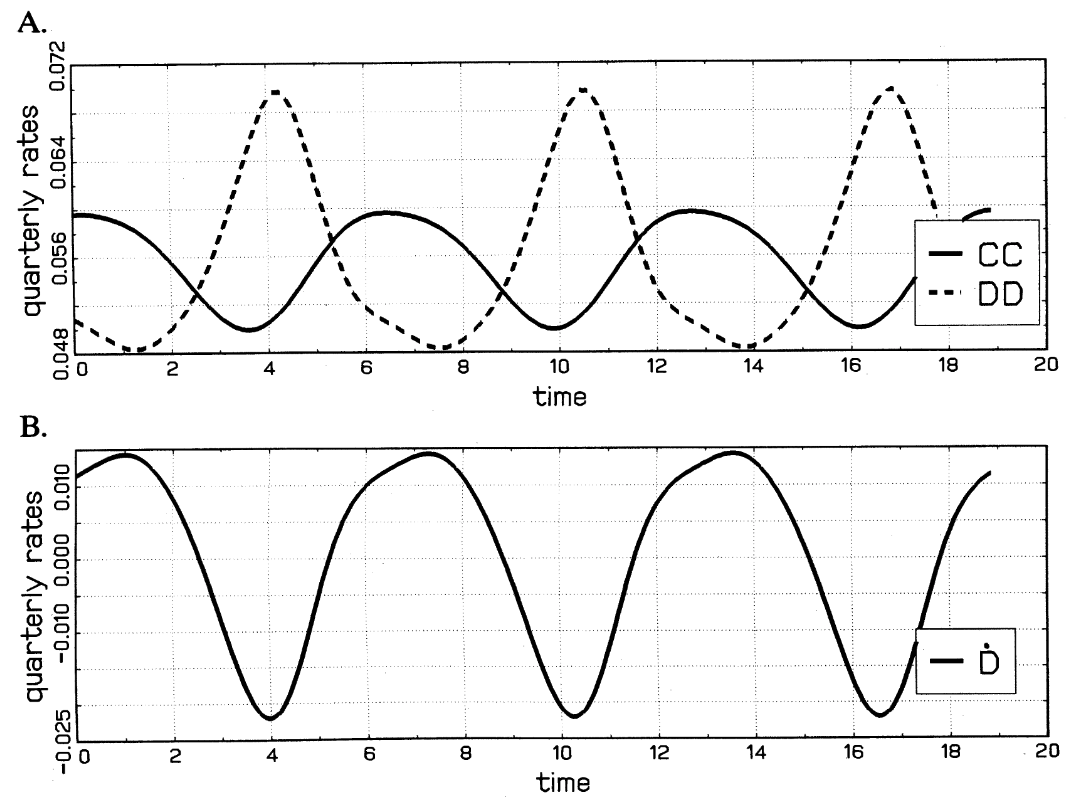
\includegraphics[scale = 0.4]{figure/Plot2.4.png}
    \caption{A.  Creation and  Destruction B. Output Growth}
    \label{plot:2.4}
    \footnotesize \textit{Notes}: The figure depicts a simulation of asymmetrical supply growth.
\end{figure}

From the plot \ref{plot:2.4}, it is evident that firms use prediction in demand to smooth job creation to avoid
big change, since they are too costly, by averaging the demand over the lifetime of a production unit. On the other
hand, destruction depends only on current conditions, thus responding only to significant deviations from the demand
prediction. It can be better understood thinking about a case in which creation rates respond only mildly to a sharp
decrease in demand, and the equilibrium price falls leading to additional destruction since older units' profits go to 0.
Indeed, destruction not only preserves but amplifies the asymmetry of demand.\paragraph{Frictionless economy}
\par
The authors culminate their study with a compelling calibration exercise using manufacturing series to exploit the
model. This entails dissecting the observed net change in employment into destruction and creation rates, as well as
applying the same approach to output production. The model is simulated for the duration of 1972:2-1983:4, with
parameters as follows: 


\begin{table}[ht]
    \centering
    \caption{Calibrated Parameters}
    \label{Tab2.1}
    \begin{tabular}{lcc}
    \hline \hline
    Variable & Symbol & Value \\
    \hline
    Interest rate & $r$ & 0.065 \\
    Depreciation rate & $\delta$ & 0.150 \\
    Rate of technical progress & $\gamma$ & 0.028 \\
    Adjustment cost parameters & $c_0$ & 0.403 \\
     & $c_1$ & 0.500 \\
    \hline
    \end{tabular}
    \end{table}
    


The technical progress is selected to attribute all the growth in employment and manufacturing to technological
advancements, setting \(\lambda\) as 2.8. The authors employ Equation \ref{eq2.9}, linking the steady state to the
lifetime of jobs and job turnover (\(CC^*\)), determining \(\overline{a}^*+7.42\) years. Utilizing this information,
they ascertain the steady state entry cost to be 0.525, equivalent to half a year's operating costs for production
units. Subsequently, they employ ordinary least squares (OLS) to retrieve the value of \(c_1\), the marginal cost of
creating a new unit, which is found to be 0.5. This aligns with a small elasticity for the creation cost function,
signifying the vulnerability of the insulation mechanism to breakdown. 
\begin{figure}
    \centering
    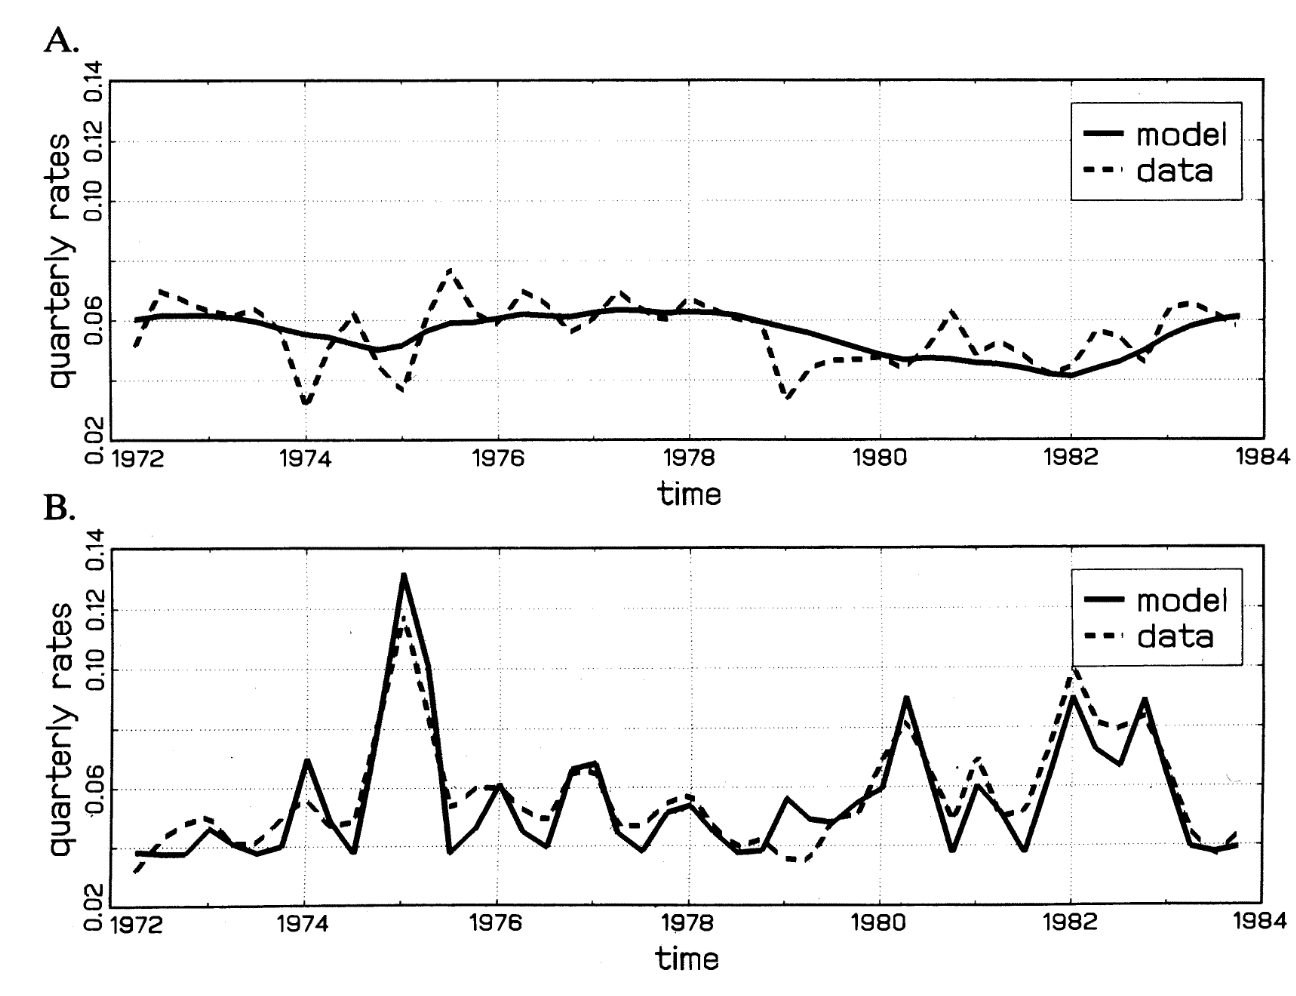
\includegraphics[scale = 0.6]{figure/Plot2.5.png}
    \caption{Figure 1. A employment driven job creation \(c_0=0.403, c_1=0.5\) B Employment job destruction \(c_0=0.403, c_1=0.5\)} 
    \label{plot:2.5}
\end{figure}
The model's simulations on employment and output, shown in Figure \ref{plot:2.5}, reveal discrepancies with actual data,
particularly in the smoother job creation trends, likely due to the model's exclusion of uncertainty. Nonetheless, it
successfully captures the volatility in job creation and destruction patterns, along with job creation's greater
symmetry, providing insights into employment and output fluctuations. The model's examination of the creation margin's
response and its impact on the destruction margin offers a baseline for understanding the cleansing effect's role in
production unit distribution.

However, the model overlooks the impact of financial frictions, which could significantly affect both creation and
destruction margins. It also entertains the notion of recessions as "pit-stops" for strategic investment, adding depth
to recession analysis. Despite the common view of procyclical labor productivity, the model, supported by
\cite{GaHam92},  suggests that recessions can indirectly boost long-term productivity through the cleansing effect.

A notable limitation is the assumption of constant marginal creation costs, which recent studies challenge, especially
for larger firms known for substantial adjustments in response to demand drops. This observed behavior in larger firms,
aligning with the model's predictions on downsizing, underscores its ability to reflect real-world dynamics despite  its
simplifications.
\subsection{Cleansing effect in \cite{OsePap17}}
The economy comprises risk-neutral firms with a constant discount rate represented by $0 < \beta < 1$. These firms
exhibit heterogeneity in productivity and net worth. They employ a production technology that relies solely on capital
(or production units) as input, featuring diminishing returns to scale.
\\
In each period, firms incur a fixed production cost denoted as $c$ to initiate production. After production, they decide
how to allocate profits for the next period. The remaining profits are invested in a risk-free asset. Firms face a
choice: they can either continue operating and reinvest their profits or exit the market, investing their entire net
worth, denoted as $e$, in the risk-free asset.
\\
Firms opt to exit the market when expected profits no longer outweigh the fixed cost $c$, or when the value of
production becomes inferior to the value they could gain by investing in the risk-free asset.
\\
The value obtained from investing in the risk-free asset is given by:
\[
q_t + \sum_{s=0}^{+\infty}\beta^s[\beta(1+r)-1]e_{t+s+1}.
\]

Notably, when the condition $\beta(1+r) \leq 1$ holds, this value simplifies to $q$. In such cases, firms are either
indifferent regarding the timing of dividend distributions or have a preference for distributing their end-of-period net
worth to shareholders or investors.
\\
In this economic model, the agents are the firms themselves, aiming to maximize their value over time by selecting an
optimal level of capital denoted as $k$. The production function, accounting for the fixed cost $c$, is expressed as
follows: $Y = Z(\theta + \epsilon)k^\alpha$.
\\
Key variables include:
\begin{itemize}
    \item $Z$: Stochastic aggregate productivity common across firms.
    \item $\theta$: Persistent firm-specific productivity shock (modeled as a Markov Chain).
    \item $\epsilon$: Firm-specific productivity shock with $\epsilon \sim \mathcal{N}(0,\delta)$.
    \item $k^\alpha$: Capital or production units, as in Caballero and Hammour (AER).
\end{itemize}

The timeline of events is as follows:

\begin{figure}[H]
    \centering
    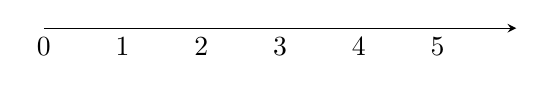
\begin{tikzpicture}
        % Draw timeline
        \draw[->,>=stealth] (0,0) -- (6,0);
        
        % Add timeline labels
        \foreach \x/\label in {0,1, 2,3, 4, 5} {
            \node[align=center, below] at (\x,0) {\label};
        }
    \end{tikzpicture}
    \caption{Timeline of Events}
\end{figure}

The sequence of events includes:
\begin{enumerate}
    \item The firm possesses knowledge of $Z,\theta,k^\alpha,e$ (where $e$ represents its endowment, different from $k$ since the firm can borrow money with $d=c+k-e$).
    \item The firm computes the optimal $k$ to maximize the expected value of the firm, with $k$ ranging from $[0,+\infty]$. If $k=0$, it indicates the firm's decision to exit.
    \item At the end of the period, the firm observes $\epsilon$ and the aggregate shock.
    \item The firm repays its debt and the fixed operating cost $(c+k-e)$, resulting in an end-of-period net worth $q$.
    \item The firm decides on the amount of dividends to distribute $(q-e')$, observes the productivity shock $\theta', Z'$, and the process restarts from step 1.
\end{enumerate}

\paragraph{Frictionless economy}
In a frictionless economy, firms have the option to borrow an amount denoted as \(c+k-e\) at the risk-free interest rate
\(r=\frac{1}{\beta}-1\). Therefore, at the start of the period, the firm's value is determined by the following
expression:

\[V_{FL} = \max_{k} E \int \max[q,\max_{e'}(q - e' + \beta V_{FL}(e',\theta', Z'))]  \,d\Phi
(\epsilon) \]
where the end of period net worth is equal to:
\[q=Z(\theta+\epsilon)k^\alpha + (1-\delta )k-(1+r)(c+k-e)\]

Under the condition of survival, it can be demonstrated that:

\[\widehat{V}_{FL}(\theta,Z) = \max_{k}E\int[Z(\theta+\epsilon)k^\alpha - (1+r)c\,d\Phi (\epsilon)] +
\beta\max[0,\widehat{V}_{FL}(\theta',Z')]\]

In the absence of market friction, firms choose to exit when their productivity reaches a certain threshold.
Specifically, they exit if \(\theta'<\underline{\theta} _{FL}(Z')\), where \(\underline{\theta}
_{FL}(Z')\) is defined as the value
for which \(\widehat{V}_{FL}(\underline{\theta}_{FL},Z')=0\).

\paragraph{Economy with Credit Market Frictions}

After production, the firm privately observes the temporary shock $\epsilon$, while financial intermediaries can only
observe it at a cost of $\mu k^\alpha$. For one-period debt contracts, financial intermediaries observe $\epsilon$ only
if the firm faces financial distress, which occurs when the private shock is insufficient to repay its debt. The terms
of the financial contract depend on the firm's net worth $e$, current productivity $\theta$, and aggregate productivity
value $Z$, all observable by both the financial intermediary and the firm at no additional cost.

\textbf{HP1 (Hypothesis 1):} The risk-free interest rate is $\beta < \frac{1}{1+r}$, which implies a lower risk-free
rate in an economy with credit frictions compared to a frictionless one. It also ensures that firms do not always
reinvest their profits.

When a firm defaults, the financial intermediary incurs verification costs and seizes all of the firm's income. The
default threshold $\overline{\epsilon}$ is determined by the equation:
\[
Z(\theta+\overline{\epsilon})k^\alpha + (1-\delta)k = (1+\widetilde{r} )(c+k+e)
\]

Default results in a zero net worth but does not necessarily force the firm to exit the market, depending on its
persistent productivity component $\theta$.

The financial intermediary lends $(c + k - e)$ to the firm only if the expected income from the loan equals the
the opportunity cost of the funds, as expressed by the inequality:
\[
(1+\widetilde{r} )(k+c+e)(1-\Phi(\overline{\epsilon}))+\int_{-\infty}^{\overline{\epsilon}}[Z(\theta+\overline{\epsilon})
k^\alpha+(1-\delta)k-\mu k^\alpha] \,d\Phi(\epsilon) \geq (1+r)(c+k+e)
\]

The financial contract is characterized by $(k,\overline{\epsilon})$. Given $Z,\theta,e$, the participation constraint
indicates the default threshold $\overline{\epsilon}$ required by the financial intermediary to lend a given amount. For
some firms, their net worth is too low for the participation constraint of the financial intermediary to be satisfied.
In fact, given $\theta, Z$, there is a unique threshold $e_b(\theta,Z)$ below which the financial intermediary
refuses to lend any amount:
\[
Z[\theta+G(\overline{\epsilon}_b )]k^\alpha+(1-\delta)k-uk_b^\alpha\Phi (\overline{\epsilon}_b)=(1+r)(k_b+c-\underline{e_b})
\]
where $\overline{\epsilon}_b$ maximizes the expected income of the financial intermediary. When the firm has a net worth
below $\underline{e_b}$, the firm defaults.

After production, the firm's end-of-period net worth is equal to:
\[
q = \begin{cases}
  Z(\theta+\overline{\epsilon})k^\alpha +(1-\delta)k-(1+\widetilde{r})(k+c-e) & \text{if } \epsilon\geq \overline{\epsilon} \\
  0 & \text{otherwise}
\end{cases}
\]
Using the default condition we can rewrite as 
\[q = \max[Zk^\alpha(\epsilon-\overline{\epsilon});0]\]

\paragraph{The firm's problem}
Define $V$ as the firm's value at the start of the period, which hinges on investment outcomes and exit decisions. If
the end-of-period net worth falls below a threshold ($q < e_b(\theta', Z')$), the firm exits. Otherwise, it compares its
continuing value to the end-of-period net worth ($q \geq e_b(\theta', Z')$) and exits if the continuing value is lower.

The firm's value function is given by:
\[
V(e,\theta,Z) = \max_{(k,\overline{\epsilon})}E\left\{\int I(q)q + (1-I(q))\max[q,\max_{e'}q-e'+\beta V(e',\theta',
\zeta')]\,d\Phi(\epsilon)\right\}
\]

Where:
\[
I(q)=
\begin{cases}
    0 & \text{if } q\geq e_b(\theta', Z')\\
    1 & \text{if } q< e_b(\theta', Z')
\end{cases}
\]

Subject to the following constraints:
\begin{enumerate}
    \item \label{con1}\[
    Z[\theta+G(\overline{\epsilon}_b )]k^\alpha+(1-\delta)k-uk_b^\alpha\Phi (\overline{\epsilon}_b)\geq(1+r)(k_b+c-
    \underline{e_b})
    \]
    \item \label{con2} \[
    q = \max[Zk^\alpha(\epsilon-\overline{\epsilon});0]
    \]
    \item \label{con3}\[
    \overline{e_b}(\theta',Z)\leq e'\leq q
    \]
\end{enumerate}

The firm aims to maximize expected dividends while complying with the financial intermediary's participation constraint
(constraint 1). Equation (constraint 2) characterizes the firm's end-of-period net worth, and
Equation (constraint 3) ensures that the
net worth
is sufficiently high to satisfy the participation constraint.
\par
Furthermore, the firm is prohibited from issuing new shares and can only augment its net worth by reinvesting profits.
This limitation presents a trade-off: increasing capital boosts production capacity but also raises the risk of default,
as the default threshold set by the financial intermediary increases with borrowed amounts.
\subsubsection{Findings}
This study investigates the complex interplay between credit frictions and the cleansing effect of recessions on firm
dynamics. By integrating models of firm dynamics with credit frictions, the authors examine how these frictions
influence the selection process for entering and exiting firms, potentially leading to the premature exit of some
high-productivity entities. Despite the impact of credit frictions on firm selection, an increase in average
productivity is observed following an aggregate productivity shock. Mirroring the dynamics in a frictionless economy, a
negative aggregate productivity shock enhances average productivity by predominantly increasing the net exit rate of
low-productivity firms. 

The analysis underscores that the extent of the recession's cleansing effect significantly depends on the steady-state
distributions of productivity and net worth among firms. The amplification in average productivity can be more
substantial than in a frictionless context, depending on the severity of credit frictions and the productivity
distribution of firms. Through calibration, the authors demonstrate that credit frictions generally mitigate the rise in
average productivity, indicating a systematic diminution in the intensity of productivity enhancement for each
percentage point increase in productivity, irrespective of the level of credit frictions and the productivity
distribution. 

Further exploration into the nature of economic shocks reveals that the type of shock critically influences the
cleansing process. Specifically, while recessions can exert a cleansing effect, the intensity of this effect is
attenuated when the downturn is triggered by a financial shock. This reduction is due to the financial shock affecting
high-productivity firms as well, suggesting a nuanced relationship between the type of economic shock and the intensity
of the cleansing effect: non-financial shocks tend to have a more significant cleansing impact compared to financial
shocks. 

Contributing to the literature on the cleansing effect of recessions, this study elucidates the role of credit frictions
in affecting the average productivity of firms by facilitating the selective exit of low-productivity firms, even under
credit constraints. It is imperative to note that the findings do not posit that recessions inherently enhance resource
allocation efficiency. On the contrary, in the presence of credit frictions, many of the exiting firms could have
remained operational in the absence of these constraints. This inefficiency is particularly evident during financial
shocks, where the exit of potentially viable firms highlights the intricate dynamics governing the cleansing effect of
recessions, emphasizing the importance of a nuanced understanding of economic downturns and their impact on firm
dynamics. 



\chapter{Theoretical model}
\section{Introduction}
This thesis presents a partial equilibrium model in which firms maximize dividends over an infinite period, under financial frictions,
investigating how those frictions can affect the saddle path of capital and dividends. Compared to \cite{OsePap17} and
\cite{CabHarm94}, this
model allows us to find a closed-form solution optimal path for dividends and capital.
The subsequent sections delve into the formulation of the flow of funds and its dynamics. Following this, the focus
shifts to scenarios  where financial frictions are present, examining their
implications on firm behavior and market outcomes. 

\section{Law of motion of capital and debt}

This model is set within a partial equilibrium framework where firms are differentiated by their productivity levels.
They have the option to fund their operations by obtaining loans from financial intermediaries, as outlined by
\cite{bernanke1995inside}, or by retaining dividends. The capital at any time \(t\) is calculated by
adjusting the capital from the previous period for depreciation (\(\delta\)), then adding gross investment (\(I\)), thus the
low of motion of capital stock is: 
\begin{align*}
    k_{t+1} &= k_{t}(1 - \delta)  + I_t  
\end{align*} 
We can rearrange  the above equation and get gross investment at time t
\begin{align}
    I_t &= k_{t+1} - k_{t}\left(1-\delta\right) \label{eq1}
\end{align} 
The \ref{eq1} equation states gross investment at time t is equal to the net capital formation plus replacement
of depreciated capital. 
The flow of funds constraint is:
\begin{align}
    I_t + R b_{t} + d_t &= f(k_t) + b_{t+1} \label{eq2}
\end{align}
where \(R\) denotes the gross interest rate and \(b_{t}\) represents the debt from period t.
The components of the flow of funds (f-of-f) at time \(t\) include:
\begin{enumerate}
    \item \(I_t\) gross investment at time t
    \item \(R b_{t}\) repayment of debts (principal and interest) 
    \item \(d_t\) dividends distributed at time t
\end{enumerate}

Conversely, the right-hand side details the sources of fund inflows:
\begin{enumerate}
    \item \(f(k_{t}) \) output at time t+1
    \item  \(b_t\) debt at time t+1
\end{enumerate}

The f-of-f constraint can be rewritten as the law of motion of debt: 
\begin{align} 
    b_{t+1} &= R b_{t} + I_{t} - S_{t}  \label{eq2'}
\end{align} 
where \(S_{t} = f(k_{t}) - d_t\) represents  earnings  retained.
This formulation clarifies that the debt level at time \(t+1\) is the sum of the repayment for the previous period's debt
(both principal and interest) and the net investment, adjusted for internal financing.

From equations \ref{eq1}, \ref{eq2'} and the definition of net worth \(n_{t+1}=k_{t+1}-b_{t+1}\), we derive the law of motion for net worth as follows:
\begin{align*}
    n_{t+1}&=k_{t+1}-b_{t+1} = k_{t}(1-\delta) + I_t - R b_{t} - I_t + S_{t} \\
    &= k_{t} - \delta k_{t} - b_{t} - r b_{t}+ S_t \\
    &= n_{t} - \delta k_{t} - r b_{t} + \left[f\left({k_t}\right) - d_t \right]
\end{align*}

The net worth or equity of the firm is given by the net worth of the previous period less the depreciated capital, less
the interest matured from the previous period augmented by the retained earnings. Therefore a firm can increase its
net worth only through increasing the retained earnings levels, thus increasing output or decreasing dividends.
Using equations \ref{eq1} and \ref{eq2}, we get the flow of funds constraint for capital:
\begin{align}
    k_{t+1}=k_{t}(1-\delta)- R b_{t} - d_t + f(k_{t})+b_{t+1} \label{eq3}
\end{align}
The above equation describes how capital evolves over time: capital at time \(t+1\) is equal to capital at time t
net of depreciation, less the repayment of debt (principal + interest), augmented by retained earnings. 

\subsection{Steady State}

From \ref{eq1}, assuming (\(k_{t+1}=k_{t}=\widehat{k}\)), we get the steady state investment:% and debt (\(b_{t-1}=b_{t} = \widehat{b}\))
 %and  for definition even dividends (\(d_t=d_{t-1}=\hat{d} \)):
\begin{align}
    \widehat{k}&=\widehat{k}\left(1-\delta\right) + \widehat{I} \nonumber\\
    \widehat{I}&=\delta \widehat{k}  \label{eq4}
\end{align}
\ref{eq4} states that in the steady state, the firm will invest only to substitute depreciated capital(\(\delta
\widehat{k}\)). From \ref{eq2'},  assuming (\(b_{t+1}=b_{t} = \widehat{b}\)) and \(d_t=d_{t+1}=\hat{d} \), we get:
\begin{align}
    \widehat{b} &= R \widehat{b} + \widehat{I} - \widehat{S} \nonumber \\
\end{align}
where \(\widehat{S} = r \widehat{b} - \widehat{I}  \), therefore:
\begin{align}
    f\left(\widehat{k}\right) - \widehat{d} - \delta \widehat{k} &= r \widehat{b} \label{eq5}
\end{align}
Equation \ref{eq5} states that in the steady state, retained earnings should be used to repay
interest over debt.
Equation \ref{eq5} can be rewritten as:
\begin{align}
    f(\widehat{k}) = \delta \cdot \widehat{k} + r \cdot \widehat{b} + \widehat{d} \label{eq5'}
\end{align}
To illustrate the equilibrium locus, one can refer to the graph in \ref{fig:steadystate3d},
which depicts the locus as defined by equation \ref{eq5'}, employing the following production function:
\begin{align}
    f(k_{t}) = Z  k_{t}^\alpha, \label{eq6} 
\end{align}
 with \(Z\) indicating the firm's productivity level, \(k_t\) indicating capital, \(0<\alpha<1\).  

\begin{figure}
    \centering
    
    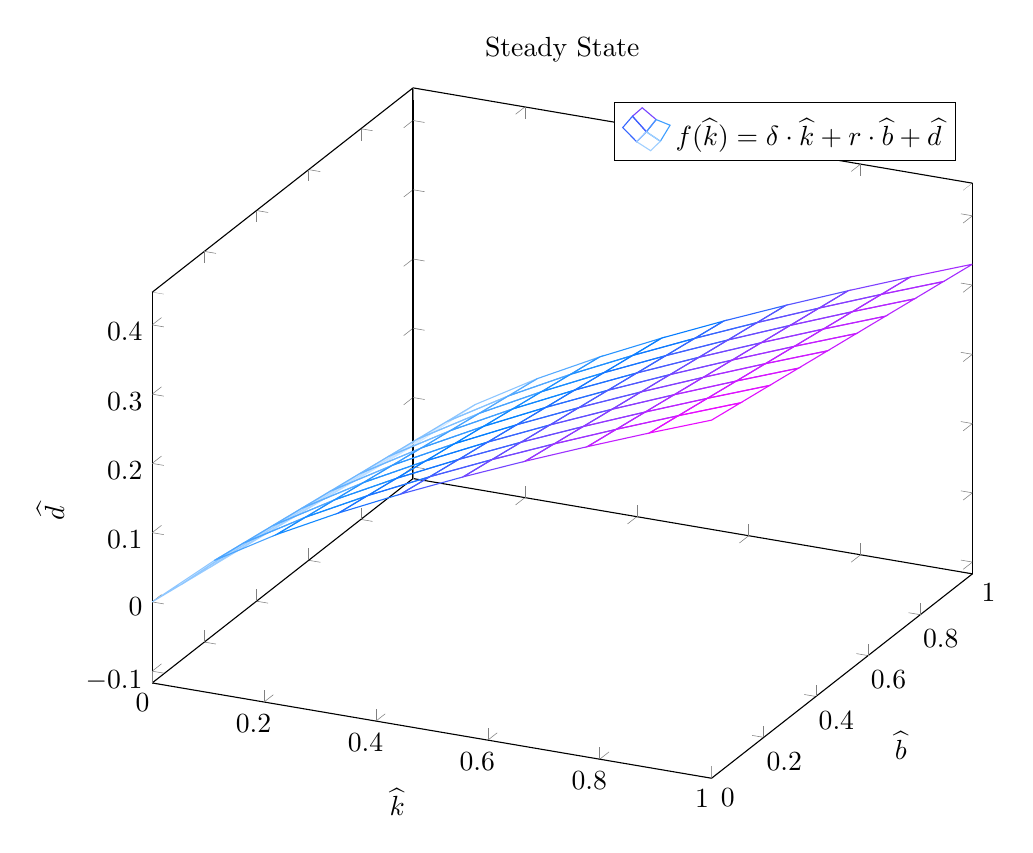
\begin{tikzpicture}
        \begin{axis}[
            title=Steady State,
            colormap/cool,
            xlabel= \(\widehat{k}\),
            ylabel= \(\widehat{b}\),
            zlabel=\(\widehat{d}\)
        ]
        \addplot3[
            mesh,
            samples=10,
            domain=0:1,
        ]
        {0.5*x^0.8-0.1*x-0.07*y};

        \addlegendentry{\(f(\widehat{k} ) = \delta \cdot \widehat{k} + r \cdot \widehat{b} + \widehat{d}\)}
        \end{axis}
    \end{tikzpicture}
    \caption{For this plot the following value has been used: \(\delta =0.1, r=0.1, \alpha=0.8, Z=0.5\)}
    \label{fig:steadystate3d}
\end{figure}

The figure illustrates the steady state relationships among debt (\(\widehat{b}\)), capital (\(\widehat{k}\)), and
dividends  (\(\widehat{d}\)) in a three-dimensional plot. The graph demonstrates how various combinations of debt and
capital influence the distribution of dividends. It is evident that, for any given level of \(\hat{k}\), a higher level of debt results in lower
dividends, as a larger portion of resources is allocated towards servicing interest payments. Conversely, the
relationship between capital and dividends, given \(\hat{b}\) is depicted as concave, highlighting an increase in dividends with higher
capital levels, under the specified model parameters: \(\delta = 0.1\), \(\alpha = 0.8\), and \(Z = 0.5\).
For example, the firm starting with initial capital \(k_0 = 0.2\) and debt \(b_0 = 0.1\), to maintain a steady state for both
capital and  debt, the dividends should be equal to \(\widehat{d} = 0.5 \times 0.2^{0.8} - 0.1 \times 0.2 - 0.1
\times 0.1\). This specific combination of \(k= 0.2\), \(b = 0.1\), \(d \approx 0.11 \) represents a stationary point in the model.
\vspace{1cm}
\subsection{Dynamics of capital}
In the
simplified scenario where a firm operates without incurring debt (\(b_t = 0\) for all \(t\)) and imposing constant and
positive dividends (\(d_t=d>0\)), the flow of funds constraint changes as follows:
\begin{align}
    I_t + d &= f(k_{t}) \\
    I_t &= S_t \label{eq7}
\end{align}
In the absence of debt, a firm's investment is solely financed through retained earnings, as
specified in equation \ref{eq7}. From \ref{eq7}, we derive the difference equation describing the evolution of capital:
\begin{align}
    \Delta{k_{t+1}} &= f(k_{t}) - d -\delta k_t +  \label{eq24}
\end{align}
Equation \autoref{eq24} presented implies that variation in capital stock depends on balance between retained earnings and
depreciated capital. Thus, for a positive increase in capital \(\Delta{k_{t+1}} > 0\), it is necessary for a company to
hold back earnings in excess of what is required to offset depreciated capital:
\begin{align*}
    f(k_{t}) - d &> \delta k_t
\end{align*}
Similarly, the reverse scenario holds as well.
To determine the steady-state level of capital, we apply the previously used production function (see equation \ref{eq6}),
setting \(k_{t+1}=k_{t}=\hat{k}\) within the difference equation (refer to equation \ref{eq24}): 
\begin{align}
    Z \hat{k}^{\alpha} - d&=  \delta \hat{k}
\end{align}
The above equation can be solved as follows:
\begin{align}
     \hat{k} &=  \left[\frac{d}{Z(1-\delta)}\right]^{\frac{1}{\alpha}} \label{eq25}
\end{align}
Recalling that the production function is monotonic and concave (\(0<\alpha<1\)), thus for a given set of parameters
(\(Z,\alpha,\delta,d\)), there is a unique steady state for capital \(\hat{k}\), defined by equation \ref{eq25}.
The slope of the phase diagram is:
\begin{align}
    \frac{\partial k_{t+1}}{\partial k_{t}} &= (1-\delta) + f^{\prime}(k_{t}) = \\
     &= (1-\delta) + \alpha Z k_{t}^{\alpha-1} \label{eq8}
\end{align}
Analysis reveals two distinct scenarios based on the derivative of capital with respect to \(k_{t}\):
\begin{enumerate}
    \item \textbf{Exploding Path When Derivative Is Greater Than 1}: If the partial derivative with respect to \(k_{t}\) is greater than 1, it suggests that small deviations from the
    steady-state level (\(\widehat{k}\)) will lead to increasing divergence rather than convergence back to
    \(\widehat{k}\). This scenario can be characterized by potentially unstable dynamics. The condition is:
    \[
    (1-\delta) + \alpha Z k_{t}^{\alpha-1} > 1, \quad \alpha Z k_{t}^{\alpha-1} > \delta, \quad k_{t} > \left(\frac{\alpha Z}{\delta}\right)^{\frac{1}{1-\alpha}}
    \]

    \item \textbf{Convergence to Steady State}: Conversely, if the derivative is less than 1, this indicates
    that deviations from the steady-state level will
    diminish over time, leading to a stable equilibrium. This scenario reflects a stable path where the system tends to
    return to its steady state following a perturbation.   The condition is:
    \[
    (1-\delta) + \alpha Z k_{t}^{\alpha-1} < 1, \quad \alpha Z k_{t}^{\alpha-1} < \delta, \quad k_{t} < \left(\frac{\alpha Z}{\delta}\right)^{\frac{1}{1-\alpha}}
    \]

\end{enumerate}

The following phase diagram represent the case \(\frac{\partial{k_t}}{\partial k_{t-1}} > 1\), using the following
parameters: \(\delta =
0.1\), \(\alpha = 0.8\), \(Z = 0.5\), and \(d = 0.8\)
\begin{figure}
    \centering
    \begin{tikzpicture}
        \begin{axis}[
            axis lines=center,
            xlabel=\(k_{t-1}\),
            ylabel={\(k_{t}\)},
            extra y ticks={0},
            extra y ticks={-0.8},
            xmin=0,
            ymin=-0.8,
        ]
        % Below the black line is defined
        \addplot [
            domain=0:5, 
            samples=100, 
            color=black,
            dotted,
        ]
        {x};
        
        % Horizontal line at y=2.5
        \draw [dotted, color=black] (axis cs:0,2.5) -- (axis cs:2.5,2.5);
        
        % Vertical line at x=2.5
        \draw [dotted, color=black] (axis cs:2.5,0) -- (axis cs:2.5,2.5);
        
        % Draw a red dot at coordinates (2.5,2.5)
        \node[draw, circle, fill=red, inner sep=2pt] at (axis cs:2.5,2.5) {};
        
        \node at (axis cs:2.5,1.8) {\(\widehat{k}\)};

        % Here the blue curve is defined with arrows
        \addplot [
            domain=0:5, 
            samples=100, 
            color=blue,
            postaction={
                decorate,
                decoration={
                    markings,
                    mark=at position 0.33 with {\arrow{<}},
                    %mark=at position 0.5 with {\arrow{>}},
                    mark=at position 0.66 with {\arrow{>}},
                }
            }
        ]
        {0.5*x^0.8 - 0.1*x + x - 0.8};
        

        \end{axis}
    \end{tikzpicture}
    \caption{The phase diagram demonstrates the evolution of capital in a debt-free scenario, with the dynamics dictated by the specific
    parameters:  depreciation rate (\(\delta =0.1\)), capital's output elasticity (\(\alpha = 0.8\)), total factor
    productivity (\( Z= 0.5\)), and fixed dividends (\(d = 0.8\)). The blue trajectory line depicts the capital accumulation
    process, calculated with the formula \( k_{t+1} = 0.5 \cdot k_{t}^{0.8} - 0.1 \cdot k_{t} + k_{t} - 0.8 \), which
    captures the interplay between capital growth through production, the diminishing returns as capital increases
    (reflected by the concavity of the curve), and the outflow due to depreciation and dividends. The steady-state
    capital (\(\widehat{k}\)), marked by a red dot, indicates the level where the economy naturally gravitates over
    time. At this point, the firm's investment is precisely calibrated to replace depreciated capital and issue
    dividends, with no additional net investment. Notably, this equilibrium is a focal point of the system; below this
    level, capital accumulates, and above it, capital stock adjusts downward, converging back to this stable point. The
    diagram serves as a visual aid to comprehend the capital dynamics within this economic framework and underscores the
    balancing act between production, depreciation, and dividend distribution in long-term capital management.
    }

\end{figure}

The graph distinctly demonstrates that when the capital at time \(t\) is below the red dot, it means that
capital is less than the steady-state capital, leading to a diminishing trajectory in the firm's capital. Conversely, if
capital is above the steady-state level, indicated by \(\widehat{k}\), the firm is overcapitalized, and the
trajectory becomes explosive, with capital increasing without bound. 
\\
If a firm's capital is less than the steady state, the outflows—such as
the replacement of depreciated capital and dividends—are disproportionately high compared to its production. This dynamic will inevitably
cause the firm's capital to go down towards zero. It's crucial to recognize that this path is predicated on the
assumption of constant dividends.
\\
Furthermore, the steeper the slope of the blue line, the higher the productivity factor \(Z\), signifying a reduced need
for capital.
\vspace{1cm}
\subsection{Dynamics of debts}
To examine the dynamics of debt, consider a scenario where capital remains constant \(k_t=k_{t+1}=\widehat{k}\), thus it is at the
steady-state level. From equation \ref{eq5'} we get the difference equation for debt:
\begin{align}
    \Delta{b_{t+1}} &= d - f(\widehat{k}) + \delta \widehat{k} + r  b_{t}  \label{eq10}
\end{align}

To derive the steady-state debt level, we'll look for the point where debt doesn't change from one period to the next,
which means  \(\Delta{b_{t+1}} = 0\). This occurs when:
\begin{align}
    d &- f(\widehat{k}) + \delta \widehat{k} + r b_{t} = 0 
\end{align}
Solving for the steady-state debt level \( \widehat{b} \), we set \( b_{t} = \widehat{b} \) and get:
\begin{align}
    d &- f(\widehat{k}) + \delta \widehat{k} + r \widehat{b} = 0 
\end{align}
 where \( f(\widehat{k}) \) is the output of the firm given the
steady-state  capital \( \widehat{k} \). Since \( f(k) \) follows a Cobb-Douglas production function \ref{eq6},  then:

\begin{align}
    d &- Z \widehat{k}^\alpha + \delta \widehat{k} + r \widehat{b} = 0
\end{align}

Isolating \( \widehat{b} \) to find the steady-state level of debt, we get:
\begin{align}
    r \widehat{b} &= Z \widehat{k}^\alpha - \delta \widehat{k} - d, \nonumber\\
    \widehat{b} &= \frac{Z \widehat{k}^\alpha - \delta \widehat{k} - d}{r}
\end{align}
This equation gives us the steady-state level of debt \( \widehat{b} \), assuming that the output of the firm is enough
to cover depreciation and dividends, with the remaining used to service debt. If output is insufficient, the
firm would need to borrow more, and the steady-state debt would be higher. If the output exceeds the depreciation and
dividends, the firm can pay down the debt, and the steady-state debt would be lower. 
Let's determine the condition for a stable path taking the partial derivatives with respect to \(b_{t-1}\):
\begin{align}
    \frac{\partial{b_t}}{\partial b_{t-1}} &= 1+r  \label{eq11} \\
\end{align}
Since \(r >0\), the partial derivative will always be greater than one, thus the slope of the
difference equation for debt will always be steeper than one. Adding a negative intercept due to positive dividends we
get that under those conditions there exists a steady state of debt. Moreover, if the debt is below the steady state, the
debt will shrink toward 0, while if the debt is over the steady state the dynamics of debt will explode toward
\(+\infty\).
\begin{figure}
    \centering
    \begin{tikzpicture}
        \begin{axis}[
            axis lines=left,
            xlabel=\(b_t\),
            ylabel={\(b_{t+1}\)},
            ymin=0,
            xmin=0,
        ]
        % Below the black line is defined
        \addplot [
            domain=0:5, 
            samples=100, 
            color=black,
            dotted,
        ]
        {x};
        % Horizontal line at y=2.5
        \draw [dotted, color=black] (axis cs:0,2.5) -- (axis cs:2.5,2.5);
        
        % Vertical line at x=2.5
        \draw [dotted, color=black] (axis cs:2.5,0) -- (axis cs:2.5,2.5);
        
        % Draw a red dot at coordinates (2.5,2.5)
        \node[draw, circle, fill=red, inner sep=2pt] at (axis cs:2.5,2.5) {};
        
        % Horizontal line at y=2.5
        \draw [dotted, color=black] (axis cs:0,1.1) -- (axis cs:1.1,1.1);
        
        % Vertical line at x=2.5
        \draw [dotted, color=black] (axis cs:1.1,0) -- (axis cs:1.1,1.1);
        
        
        
        % Here the blue curve is defined with arrows
        \addplot [
            domain=0:5, 
            samples=100, 
            color=blue,
            postaction={
                decorate,
                decoration={
                    markings,
                    mark=at position 0.1 with {\arrow{<}},
                    %mark=at position 0.5 with {\arrow{>}},
                    mark=at position 0.3 with {\arrow{>}},
                }
            }
        ]
        {-0.5*3^0.8 + 0.1*3 + 1.1*x + 0.8};
        % Draw a red dot at coordinates (2.5,2.5)
        \node[draw, circle, fill=green, inner sep=2pt] at (axis cs:1.1,1.1) {};

        \end{axis}
    \end{tikzpicture}
    \caption{The phase diagram dynamically visualizes the firm's debt trajectory given a static capital stock ($\Delta k = 0$),
    operationalized within a model characterized by the parameters $\delta = 0.1$ (depreciation rate), $r = 0.1$
    (interest rate), $\alpha = 0.8$ (capital output elasticity), $Z = 0.5$ (total factor productivity), $d = 0.8$
    (constant dividend payout), and a steady-state capital ($\widehat{k} = 3$). The blue line embodies the trajectory of
    debt, guided by  the finite difference equation $b_{t+1} = (1+r) \cdot b_{t} - (f(\widehat{k}) -
    \delta \widehat{k} - d)$, where $f(\widehat{k})$ denotes the firm's output at the steady state of capital. This
    equation encapsulates the interplay between the interest on existing debt and the firm's obligations due to
    dividends and depreciation. The red dot marks the threshold beyond which debt cannot exceed capital, effectively serving
    as a limit 
    on debt. The green dot
    represents the equilibrium or steady-state debt level, where the firm's financial obligations are perfectly balanced
    with its repayment capacity. The distance between the red and green dots illustrates the magnitude of the firm's
    equity buffer, serving as a measure of financial health and resilience against market fluctuations. This diagram is
    pivotal in understanding how dividend policies and productivity rates interlink to shape the firm's leverage
    strategy and long-term financial stability.}
    \label{fig:ph_k}
\end{figure}
The phase diagram \autoref{fig:ph_k} illustrates the relationship between a firm's current debt (\(b_t\)) and its capacity for future operations
(\(k_{t+1}\)), within the context of constant dividends. The steady state is indicated by the red dot, signifying the
juncture at which the firm's output is precisely adequate to cover dividends, depreciation, and interest on its
steady-state debt. %r
In essence, the graph conveys how steady-state conditions are shaped by dividend policy and productivity, with the
former influencing the firm's financial leverage and the latter determining its capital efficiency. 




\section{Ramsey-Cass-Kooopmans reinterpreted}
This section outlines the intertemporal maximization problem faced by the firm in the absence of debt, which is a
Ramsey-Cass-Kooopmans revisited model, where there is a firm that seeks to maximize the utility of dividends consumption of the shareholders.
The objective function is:
\[V_0 = \sum_{t=0}^{+\infty}{\beta^t U(d_t)},\]
where \(U^{\prime}>0, U^{\prime \prime}<0\).
\subsection{Steady State derivation}
Let's assume that the firm's investment is entirely financed by equity (\(b_t=0\)  for all \(t\)), this leads to a simplified flow-of-funds constraint equation:
\begin{align}
    k_{t+1} = k_{t}(1 - \delta) + f(k_{t}) - d_{t}.  \label{eq13}
\end{align}
The maximization problem is tackled using a Lagrangian method, where the Lagrangian is defined as:
\[L_0 = \sum_{t=0}^{+\infty}\left[{\beta^t U(d_t) - \beta^t \lambda_t\left[k_{t+1} - k_{t}(1 - \delta) - f(k_t) + d_t\right]}\right].\]

The first-order conditions for \(d_{t}\), \(k_{t}\), for all periods \(t=0,1,\ldots\) yield:
\[
U^{\prime}(d_{t}) = \lambda_t, \quad \forall t,
\]
\[
\beta^t \lambda_t = \beta^{t+1} \lambda_{t+1}[f^{\prime}(k_{t+1}) + (1-\delta)], \quad \forall t,
\]


This approach delineates the optimal strategy for dividend distribution and capital allocation in a debt-free
case.
In the infinite horizon model, the transversality condition reads:
\begin{align}
    \lim _{t \rightarrow \infty} \beta^T U^{\prime}\left(d_{t}\right) k_{T+1}=0 \label{eq26}
\end{align}
From these first-order conditions (FOCs), we derive the Euler equation for dividends:
\begin{align}
    U^{\prime}(d_{t}) = \beta U^{\prime}(d_{t+1})[f^{\prime}(k_{t+1}) + (1-\delta)]  \label{eq14}
\end{align}
indicating that the marginal utility of distributing 1 unit of output as dividends at time \(t\) should match the discounted marginal
utility of not distributing  dividends in t,saving, investing in t, using the additional capital to produce and
distribute the corresponding dividends at time t+1.
\paragraph{Steady state condition for dividends}
Imposing the steady state condition for dividends \( d_t = d_{t+1} = \widehat{d} \) in \ref{eq14} , we
equate the marginal  utilities across two consecutive periods:
\begin{align}
    U^{\prime}(d_t) &= U^{\prime}(d_{t+1}), \nonumber \\
    \frac{1}{\beta} = f^{\prime}(k_{t+1}) + (1-\delta),\label{eq27}
\end{align}
This condition is satisfied if:
\begin{align}
    f^{\prime}(k_{t+1}) &= \frac{1}{\beta} - (1-\delta), 
\end{align}
Using the Cobb Douglas production function and take the derivative respect to capital, we get:
\begin{align}
    f^{\prime}(k_{t+1}) &= Z \alpha k^{\alpha-1}_{t+1},  \label{eq15'}
\end{align}
From \ref{eq27}, we get: 
\begin{align}
    \frac{1}{\beta}&=1-\delta+Z\alpha k^{\alpha-1},\nonumber \\
    Z\alpha k^{\alpha-1} &+(1-\delta)\beta=1, \nonumber \\
    \widehat{k} &= \left[\frac{\alpha \beta Z}{1 - \beta\left(1-\delta\right)}\right]^{\frac{1}{1-\alpha}}.  \label{eq16}
\end{align}
The locus of points on the (\(k_t,d_t\)) plane such that dividends are constant is therefore
\(k_t=\hat{k}\), whose representation in the vertical line in figure \ref{fig:ph_d_k_nod_1}.
\paragraph{Steady state condition for capital}
Imposing steady state condition for capital (\(k_t = k_{t-1} = \widehat{k}\)) in the law of motion of capital \ref{eq13} we
get:
\begin{align}
    \widehat{d} & = f(k_t) - \delta k_t  \label{eq17}
\end{align}
This locus represents the set of points where the capital stock remains constant over time. Hence, we can determine the
level of dividends that ensures both capital and dividends are maintained at steady-state levels. By incorporating the
steady-state level of capital  from Equation \ref{eq16} and the production function from Equation \ref{eq6} into the equilibrium
condition for capital from Equation \ref{eq17}, the steady-state level of dividends, denoted as \( \widehat{d} \), can be
deduced:

\begin{align}
    \widehat{d} &= Z \left( \frac{\alpha \beta Z}{1 - \beta(1 - \delta)} \right)^{\frac{\alpha}{1 - \alpha}} - \delta \left( \frac{\alpha \beta Z}{1 - \beta(1 - \delta)} \right)^{\frac{1}{1 - \alpha}}
\end{align}



In this manner, we ascertain the steady-state levels for both capital and dividends.
\subsection{Phase diagram}

In this section, we will plot the phase diagram for capital and dividends exploiting steady-state conditions for capital and
dividends. 
\begin{figure}
    \centering
    \begin{tikzpicture}
        \begin{axis}[
            axis lines=middle, % sets the position of the axes
            xlabel=\(k_t\),
            ylabel=\(d_t\),
            ymin=0, xmin=0,
            xmax=5, ymax=5,
            ticks=none, % removes ticks on axes
            clip=false,
            every axis plot post/.style={thick}
        ]
        
        % Vertical line at k hat
        \draw  (axis cs:1.8,0) -- (axis cs:1.8,5);
        \node at (axis cs:2,5.5) {\(\Delta d_t = 0\)};
        \node at (axis cs:1.8,-0.5) {\(\hat{k}\)};
        
        % Arrows
        % Upwards arrows
        \draw [-{Latex[length=3mm]}] (axis cs:1,1) -- (axis cs:1,2);
    
        % Downwards arrows
        \draw [{Latex[length=3mm]}-] (axis cs:3,1) -- (axis cs:3,2);

        \end{axis}
    \end{tikzpicture}
    \caption{The phase diagram illustrates locus of points such that \(d_t=d_{t-1}\). The vertical line at \( \hat{k} \) represents the steady-state level of capital, where
    the rate of change in dividends \( \Delta d_t \) is zero. To the left of \( \hat{k} \), where capital is below its
    steady-state level, the firm increases dividend payments. Conversely, to the right of \( \hat{k} \), where capital
    exceeds the steady state, dividend payments decrease.}
    \label{fig:ph_d_k_nod_1}
\end{figure}

The graph \autoref{fig:ph_d_k_nod_1} portrays the dynamics of dividends (\(d_t\)) in relation to the capital (\(k_t\)) of a firm, with a
particular focus on the behavior when capital is below or above the steady-state level,  denoted by \(\hat{k}\).

When the capital is below the steady-state level (\(k_t < \hat{k}\)), thus on the left of the vertical line, for the
firm is optimal to increase dividends over time (\(d_t<d_{t+1}\)) as represented by the arrow pointing upward. When instead
(\(k_t > \hat{k}\)), dividends must shrink over time (\(d_t>d_{t+1}\)).
Lets look at the locus in which capital is stationary \(\Delta k = 0 \) is given by the f-of-f constraint \ref{eq17}:
\begin{align}
    d_t & = f(k_t) - \delta k_t
\end{align}
In our case, as obtained in the above section, the locus in which capital is stationary becomes \ref{eq17}:
\begin{align}
    d_t &=Z k^{\alpha}_t-\delta k_t
\end{align}

This function starts at the origin since (\(f(0)=0\)), with a maximum in \(\underline{k}\) (defined as capital level
such that \(f^{\prime}(\underline{k})=\delta\)). The level of capital \(\underline{k}\) is:
\begin{align}
    \underline{k} &= \left[\frac{\alpha Z}{\delta}\right]^{\frac{1}{1-\alpha}}  \label{eq19}
\end{align}
It is easy to see that \(\hat{k}<\underline{k}\):
\begin{align*}
    \frac{\alpha \beta Z}{1-\beta+\beta \delta}&<\frac{\alpha Z}{\delta},\\
    \frac{\beta}{1-\beta+\beta \delta}&<\frac{1}{\delta},\\
    \beta \delta &<1-\beta + \beta \delta, \\
    1-\beta&>0 \\
    \text{for definition} \quad \blacksquare 
\end{align*}
We denote \(\bar{k}\) the capital level such that \(d_t=0\), thus it's obtained by solving \(f(\bar{k}) -\delta
\bar{k} = 0\), using the Cobb-Douglas production function \ref{eq6}, we get:
\begin{align}
    Z \bar{k}^{\alpha} &= \delta \bar{k}, \nonumber\\
    \bar{k}&=\left[\frac{Z}{\delta}\right]^{\frac{1}{1-\alpha}}
\end{align}
It is easy to see that \(\underline{k}<\bar{k}\), since:
\begin{align}
    \left[\frac{Z}{\delta}\right]^{\frac{1}{1-\alpha}}&>\left[\frac{\alpha Z}{\delta}\right]^{\frac{1}{1-\alpha}},\nonumber\\
    \frac{Z}{\delta}&>\frac{\alpha Z}{\delta}, \nonumber \\
    1&>\alpha \nonumber \\
    \text{for definition} \quad \blacksquare 
\end{align}
Considering transitivity, the sequence for \(\underline{k}, \hat{k}, \bar{k}\) is:
\begin{align*}
    \hat{k} < \underline{k} < \bar{k}
\end{align*}
\begin{figure}
    \centering
    \begin{tikzpicture}
        \begin{axis}[
            axis lines=middle, % sets the position of the axes
            xlabel=\(k_t\),
            ylabel=\(d_t\),
            xmin=0, ymin=0,
            xmax=5, ymax=5,
            ticks=none, % removes ticks on axes
            clip=false,
            axis on top=true
        ]
        
        % Parabolic curve
        \addplot [
            domain=0:4, 
            samples=100, 
            thick,
        ]
        {-x^2 + 4*x};
        
        % Vertical line at k hat

        \node at (axis cs:3.5,3.5) {\(\Delta k_t = 0\)};

        
        % Arrows on the left side
        \draw [-{Stealth[bend]}]  (axis cs:0.5,1)--(axis cs:1,1);
        \draw [-{Stealth[bend]}]  (axis cs:0.8,4) -- (axis cs:0.5,4);
        
        % Arrows on the right side
        \draw [-{Stealth[bend]}]  (axis cs:2.5,1)--(axis cs:3,1);
        \draw [-{Stealth[bend]}]  (axis cs:4,4) -- (axis cs:3.5,4);
        \node at (axis cs:2,-0.2) {\(\underline{k}\)};
        \node at (axis cs:4,-0.2) {\(\bar{k}\)};

        %vertical line at maximum
        \draw [dashed] (axis cs:2,0) -- (axis cs:2,4);
        \end{axis}
    \end{tikzpicture}
    \caption{This phase diagram displays the set of points at which the capital stock \( k_t \) is
    unchanging from one period to the next (\( k_t = k_{t-1} \)). The capital level at \( \underline{k} \) represents the
    maximum sustainable dividend payout without affecting the capital stock. Arrows above the curve pointing leftward
    indicate a reduction in capital resulting from dividend levels that exceed the sustainable steady state, while
    arrows pointing to the right below the curve signify the accumulation of capital due to dividend levels that are
    below the steady state, leading to an increase in capital stock over time. 
    }
    \label{fig:ph_d_k_nod}
\end{figure}

For a given level of capital \(k_0 \in [0,\bar{k}]\), the corresponding dividends level that
guarantee the stationarity of capital is:
\begin{align*}
    d_0 &= f(k_0) -\delta k_0
\end{align*}
If the firm distributes more dividends than \(d_0\) the capital stock must decrease over time: since
dividends are too high the firm is consuming part of her capital. More precisely the firm is distributing more dividends than
\(d_0\), which guarantees that the difference between production, and dividends is exactly equal to the replacement of
depreciated capital.
This behavior is represented by the arrows above the curve pointing to the left. If the firm distributes less
dividends than \(d_0\), the opposite happens: the firm increases its capital since there is a positive net
investment. This behavior is represented by
the arrows below the curve pointing toward the right. 

\paragraph{Steady state for capital and dividends}
Plotting both loci we get a phase diagram that represents the condition for stationarity. 
\begin{figure}
    \centering
    \begin{tikzpicture}
        \begin{axis}[
            axis lines=middle, % sets the position of the axes
            xlabel=\(k_t\),
            ylabel=\(d_t\),
            xmin=0, ymin=0,
            xmax=5, ymax=5,
            ticks=none, % removes ticks on axes
            clip=false,
            axis on top=true
        ]
        
        % Parabolic curve
        \addplot [
            domain=0:4, 
            samples=100, 
            thick,
        ]
        {-x^2 + 4*x};
        
        % Arrows
       
        
        % Vertical line at k hat
        \draw [dashed] (axis cs:2,0) -- (axis cs:2,4);
        \node at (axis cs:2.5,4.5) {\(\Delta d_t = 0\)};
        \node at (axis cs:3.5,3.5) {\(\Delta k_t = 0\)};
        \node at (axis cs:4,-0.2) {\(\bar{k} \)};

        \draw  (axis cs:1.8,0) -- (axis cs:1.8,5);

        \node at (axis cs:1.8,-0.2) {\(\hat{k} \)};
        % Arrows on the left side
        \draw [-{Stealth[bend]}]  (axis cs:1.3,1)--(axis cs:1.8,1);
        \draw [-{Stealth[bend]}]  (axis cs:0.8,3) -- (axis cs:0.3,3);
        
        % Arrows on the right side
        \draw [-{Stealth[bend]}]  (axis cs:2.5,1)--(axis cs:3,1);
        \draw [-{Stealth[bend]}]  (axis cs:4,3) -- (axis cs:3.5,3);
        
        % Arrows
        % Upwards arrows
        \draw [-{Stealth[bend]}]  (axis cs:0.8,3) -- (axis cs:0.8,3.5);
        \draw [-{Stealth[bend]}]  (axis cs:1.3,1) -- (axis cs:1.3,1.5);
        \draw [-{Stealth[bend]}]  (axis cs:2.5,1) -- (axis cs:2.5,0.5);
        \draw [-{Stealth[bend]}]  (axis cs:4,3) -- (axis cs:4,2.5);
        
        % Vertical line at k hat
        \draw [dashed] (axis cs:1,0) -- (axis cs:1,5);
        \node at (axis cs:0.8,2) {A};
        \node at (axis cs:1,-0.2) {\(k_0\)};
        \draw [dashed] (axis cs:1,0) -- (axis cs:1,5);
        
        % Draw a green dot at coordinates (1.1,1.1)
        \draw [-{Stealth[bend]}, color=blue]  (axis cs:1,2) -- (axis cs:1.76,3.87);
        \node[draw, circle, fill=green, inner sep=2pt] at (axis cs:1.81,3.96) {};
        \node[draw, circle, fill=green, inner sep=2pt] at (axis cs:1,2) {};
        \node at (axis cs:1.7,4.2) {B};
        
        \node at (axis cs:2,-0.2) {\(\underline{k}\)};
        \end{axis}
    \end{tikzpicture}
    \caption{The phase diagram visualizes the relationship between dividends and capital. The vertical line marks
    where the dividend level remains constant, and the solid concave curve traces where the capital remains constant.
    Point B indicates the equilibrium where both dividends and capital are stationary, with the steady-state capital at
    \( \hat{k} \). This value of \( \hat{k} \) is notably lower than \( \underline{k} \), which is the capital level
    that would maximize dividends while maintaining a steady capital stock. \( \bar{k} \) represents the capital
    quantity at which the system reaches a stationary state for k with zero dividends. The arrows illustrates the dynamics of dividends and capital in case of the firm finding itself outside the stable
    loci. Point A is a possible starting point (\(k_0,d_0\)). 
    The blue arrows indicate a potential trajectory, known as a saddlepath, leading towards the saddlepoint B. 
    }
    \label{fig:ph_d_nodebt}
\end{figure}
Notice that there exits 3 steady states: one at the origin due to the assumption \(f(0)=0\), the point \((\bar{k};0)\),
and finally point B \(=(\hat{k},\hat{d})\). Point B was obtained by equations \ref{eq16} and \ref{eq17} and represented the point in
which dividends and capital are at a steady state, and both are strictly positive. This point is a saddlepoint.
The blue line depicts a possible saddlepath towards B. Starting at A, the firm chooses exactly the dividend level that
leads to the stationary point B. This path not only fulfills the difference equations \ref{eq14} and \ref{eq17}, but
also, the transversality condition \ref{eq26}
Indeed as \(t \rightarrow \infty\), capital and dividends approach their steady-state level which are both positive and
finite, thus the marginal utility of dividends at \(\hat{d}\) is also finite, hence \ref{eq26} is valid.

To conclude, this section has outlined the derivation of steady-state levels for capital and dividends, and these
conditions have been visually represented in a phase diagram. The upcoming section will undertake a similar analysis but
will incorporate debt and financial friction into the model. Additionally, it is important to note that in the steady
state, where output \(\hat{y}\) is given by \(f(\hat{k})\), the production level is exclusively influenced by the
productivity parameter \(Z\), signifying that financial elements do not alter the fundamental connection between the
production function and output. 

\section{Introducing financial frictions}
In this section we tackle the maximization problem of the firm, introducing the possibility of financing through
debt and two types of financial frictions. The first financial friction is a financing constraint, which implies fixed
leverage for the firm. The second financial friction is introducing a participation
constraint with monitoring cost for the financial intermediaries. The goal is to understand how those frictions
affect the steady state of capital and dividends.

\subsection{Participation constraint of the financial intermediaries } 
The subsection delves into the constraints facing financial intermediaries within the model. Initially, the model assumed an exogenous
interest rate, unaffected by the volume of debt, leading to an unrealistic scenario where interest rates remain
constant.  To address this,  the model incorporates a financial market in which the interest rate is set based on
market-clearing conditions, with financial intermediaries functioning in a perfectly competitive environment aimed at
profit maximization. 

According to \cite{BerGer86}, lending should yield a profit equivalent to the opportunity cost. Lenders earn
interest plus the principal if borrowers repay successfully (with probability \(p\)) or acquire the firm's production
assets (net of monitoring cost: \(1-\mu\)) in case of bankruptcy. Moreover, \((1-\mu)f(k_t)\)represents monitoring cost.
The lender's participation constraint is:
\begin{align*}
    R_t \cdot b_t p + (1-p) \mu f(k_t) = R_f b_t, \
\end{align*}

where \(R_f\) represents the risk-free rate, the opportunity cost of lending. This
framework allows for  the derivation of the interest rate as a function of \(p\),\(f(k_t)\),\(\mu\),\(\b_t\) and \(R_f\).

The participation constraint can be rewritten as:
\begin{align}
    R_t=\frac{R_f}{p}  -\frac{ 1-p }{ p }\frac{\mu f(k_t)}{b_t}. \label{eq21}
\end{align}

Investigating the asymptotic behavior of \( R_t \) with respect to \( p \) provides critical economic insights.
Specifically, as \( p \rightarrow 0 \), indicating an increasingly likely default, \( R_t \) escalates without bound,
reflecting the infinitely rising premium a lender would require to counterbalance the heightened risk. Conversely, as \(
p \rightarrow 1 \), the default risk vanishes, and \( R_t \) converges to \( R_f \), the risk-free rate, consonant with
the absence of default risk necessitating no premium above the risk-free return. 
When examining the behavior of the interest rate formula as the debt amount \(b_t\) trends towards infinity, the resulting limit is given by:

\[
\lim_{{b_t \rightarrow +\infty}} \frac{R_f}{p} - \frac{1-p}{p}\frac{\mu f(k_t)}{b_t} = \frac{R_f}{p}
\]

As the denominator \(b_t\), representing the total
debt, increases without bound, the term involving the firm's productive output adjusted for recovery rate (\(\mu
f(k_t)/b_t\)) diminishes to zero. This indicates that, in scenarios of very large debt volumes, the fraction of
recoverable assets (\(\mu f(k_t)\)) compared to the outstanding debt becomes negligible in determining the interest rate
\(R_t\).

Therefore, under such conditions, the interest rate formula simplifies to \(\frac{R_f}{p}\), underscoring that the
loan's interest rate is fundamentally determined by the risk-free rate adjusted for the probability of successful
repayment \(p\), independent of the firm's asset recoverability or productivity levels. This elucidates an important
economic principle: for vast sums of debt, the critical factors shaping lending rates pivot away from the specifics of
asset recovery towards broader financial metrics—namely, the prevailing risk-free rate and the inherent risk of default.



The breakeven threshold for \( R_t \), where the return on the loan is nonnegative, is formalized by the condition:

\begin{align}
    R_f b_t \geq b_t  p +(1-p) \mu  f(k_t). 
\end{align}
This inequality dictates that to achieve a return rate on the loan that is greater than or equal to one, the opportunity
cost of capital must be greater than expected profit from the firm's production, adjusted for default probability and asset
recoverability post-default. This ensures the lender receives a return that compensates for the risk undertaken,
juxtaposed with the risk-free alternative.
Let's present a specific scenario for clarity: Imagine we have a constant capital level \(k\), and the recovery rate in
case of default \(\mu\) is complete, meaning \(\mu=1\). In this instance, the depreciation rate \(\delta\) is 0.1, the
output elasticity of capital \(\alpha\) is set at 0.8, while the technology factor \(Z\) is 0.5. Additionally, the
firm's dividends level \(d\) is 0.8, and the capital stock at time \(t\), \(k_t\), equals 4. The risk-free rate \(R_f\) is given as
1.05.

Within this framework, consider two firms that are identical in every aspect except for their probability of returning
profit, denoted by \(p\). For the first firm, \(p\) is 0.95, suggesting a 5\% default risk. For the second firm, \(p\)
drops to 0.9, indicating a higher default risk of 10\%. The graphical representation suggests that as debt levels
increase, so do interest rates, reflecting the risk-return dilemma for lenders. A higher risk profile, denoted by a more
elevated red line necessitates greater returns to compensate for default risks. It's important to note that while the
the graph assumes constant capital, real-world scenarios often see debt increases leading to higher capital and,
consequently, greater production capacities.

The analysis indicates that the blue curve, representing the rate of return for a riskier firm, is positioned above the red curve under a specific condition:

\begin{equation}
    \mu f(k_t) < R_f b_t
\end{equation}

This condition implies that the net output from employing capital \(k_t\), after accounting for monitoring costs, must
be less than the opportunity cost associated with lending the sum \(b_t\). Should this not hold true, firms with a
higher risk profile would end up incurring lower interest charges on their loans. To elucidate, consider the following
scenario where \(p_h\),  denoting the probability of avoiding default for the less risky firm, is higher than \(p_l\),
the corresponding probability for the riskier firm. All other factors are assumed to remain constant across both firms:

\begin{align*}
    \frac{R_f}{p_h}  -\frac{1 - p_h}{p_h}\frac{\mu f(k_t)}{b_t} &< \frac{R_f}{p_l} - \frac{1 - p_l}{p_l}\frac{\mu f(k_t)}{b_t}, \\
    \left[R_f - (1 - p_h) \mu \frac{f(k_t)}{b_t}\right] p_l &< \left[R_f - (1 - p_l) \mu \frac{f(k_t)}{b_t}\right] p_h,\\
    \left[-(1 - p_h)p_l + (1 - p_l)p_h\right] \mu \frac{f(k_t)}{b_t} &< R_f (p_h - p_l),\\
    \mu \frac{f(k_t)}{b_t} &< R_f,\\
    \mu f(k_t) &< R_f b_t.
\end{align*}

This sequence of steps demonstrates that for the gross rate of return on loans to be positioned favorably for riskier firms,
the expected output from the investment (after subtracting monitoring costs) must not exceed the lending opportunity
cost.

\begin{figure}
    \centering
    \begin{tikzpicture}
        \begin{axis}[
            domain=0:5, y domain=0:1.5, % Corrected the domain specification
            ymin=0, ymax=, % Set the y-axis limits
            xmin=0, xmax=5, % Set the x-axis limits
            axis lines=left,
            xlabel=\(b_t\),
            ylabel={\(r_t\)},
        ];
        % Below the black line is defined
        % Horizontal line at y=2.5 is outside the y-axis limit and should be removed or adjusted
        
        % Vertical line at x=2.5 is outside the y-axis limit and should be removed or adjusted
        
        % Draw a red dot at coordinates (2.5,2.5) is outside the y-axis limit and should be removed or adjusted
        
        % Horizontal line at y=1.1
        \draw [dotted, color=black] (axis cs:0,1.1) -- (axis cs:1.1,1.1);
        
        % Vertical line at x=1.1
        %\draw [dotted, color=black] (axis cs:1.5,0) -- (axis cs:1.5,1.1);
        
        % Here the blue curve is defined with arrows
        \addplot [
             % Corrected the domain specification
            samples=100, 
            color=blue,
            postaction={
                decorate,
                decoration={
                    markings,
                    mark=at position 0.1 with {\arrow{>}},
                    %mark=at position 0.5 with {\arrow{>}}, % Commented out as not needed
                    mark=at position 0.3 with {\arrow{<}},
                }
            }
        ]
        {(1.05/0.90)-((0.1/0.9)*(0.5*((4)^0.8))/x)-1};

        \addplot [
             % Corrected the domain specification
            samples=100, 
            color=red,
            postaction={
                decorate,
                decoration={
                    markings,
                    mark=at position 0.1 with {\arrow{>}},
                    %mark=at position 0.5 with {\arrow{>}}, % Commented out as not needed
                    mark=at position 0.3 with {\arrow{<}},
                }
            }
        ]
        {(1.05/0.95)-((0.05/0.95)*(0.5*((4)^0.8))/x)-1};
        
        % Draw a green dot at coordinates (1.1,1.1)
        \node[draw, circle, fill=green, inner sep=2pt] at (axis cs:1.1,1.1) {};

        \end{axis}
    \end{tikzpicture}
    \caption{The figure presents a graphical analysis of the returns on loans as a function of the loan amount under a fixed capital level of 
    \(k=4\). The red curve models the scenario where the default risk probability is 
    \(1-p=0.05\)
    , implying a 5\% chance of default, while the blue curve corresponds to a higher default risk at 
    \(1-p=0.1\), a 10\% chance of default. Both curves reflect the increased interest rates required to compensate for
    the heightened risk as the debt stock grows. Notably, the opportunity cost of capital is maintained at 0.05 for the
    red one, while at 0.1 for the higher risk curve.
    }
    \label{plot:part_constraint_r_lavarge}
\end{figure}

The graph \ref{plot:part_constraint_r_lavarge} captures the dynamics between the debt stock \(b_t\) and the interest
rate applied to the loan \(r_t\). An
increase in the debt stock leads to a rise in the interest rate, reflecting the augmented risk
perceived by lenders. Displayed are two distinct lines: one representing a riskier loan with a higher probability of
default and the other indicating a safer loan with a lower default probability. As anticipated, the riskier loan
scenario is characterized by a curve that lies above, dictating higher interest rates, if \(\mu f(k_t) < R_f b_t\) holds. 

An alternative approach to illustrating the participation constraint of financial intermediaries involves graphing the gross
interest rate, \( R \), against the ratio of output to debt, \( \frac{f(k)}{b} \), directly. 
\begin{figure}
    \centering
    \begin{tikzpicture}
        \begin{axis}[
            domain=0:5, y domain=0:1.5, % Corrected the domain specification
            ymin=0, % Set the y-axis limits
            xmin=0, xmax=5, % Set the x-axis limits
            axis lines=left,
            xlabel=\(f(k_t)/b_t\),
            ylabel={\(r_t\)},
        ];
        % Below the black line is defined
        % Horizontal line at y=2.5 is outside the y-axis limit and should be removed or adjusted
        
        % Vertical line at x=2.5 is outside the y-axis limit and should be removed or adjusted
        
        % Draw a red dot at coordinates (2.5,2.5) is outside the y-axis limit and should be removed or adjusted
        
        % Horizontal line at y=1.1
        \draw [dotted, color=black] (axis cs:0,1.1) -- (axis cs:1.1,1.1);
        
        % Vertical line at x=1.1
        \draw [dotted, color=black] (axis cs:1.05,0) -- (axis cs:1.05,1);
        
        % Here the blue curve is defined with arrows
        \addplot [
             % Corrected the domain specification
            samples=100, 
            color=blue,
            postaction={
                decorate,
                decoration={
                    markings,
                    % mark=at position 0.1 with {\arrow{>}},
                    mark=at position 0.5 with {\arrow{>}}, % Commented out as not needed
                    % mark=at position 0.3 with {\arrow{<}},
                }
            }
        ]
        {(1.05/0.90)-((0.1/0.9)*x)-1};

        \addplot [
             % Corrected the domain specification
            samples=100, 
            color=red,
            postaction={
                decorate,
                decoration={
                    markings,
                    % mark=at position 0.1 with {\arrow{>}},
                    mark=at position 0.5 with {\arrow{>}}, % Commented out as not needed
                    % mark=at position 0.3 with {\arrow{<}},
                }
            }
        ]
        {(1.05/0.95)-((0.05/0.95)*x)-1};
        
        % Draw a green dot at coordinates (1.1,1.1)
        \node[draw, circle, fill=green, inner sep=2pt] at (axis cs:1.1,1.1) {};

        \end{axis}
    \end{tikzpicture}
    \caption{The figure presents a graphical analysis of the returns on loans as a function of the production over the
    debt level. The red curve models the scenario where the default risk probability is 
    \(1-p=0.05\)
    , implying a 5\% chance of default, while the blue curve corresponds to a higher default risk at 
    \(1-p=0.1\), a 10\% chance of default. Both curves reflect the increased interest rates required to compensate for
    the heightened risk as the production-debt ratio grows. Notably, the opportunity cost of capital is maintained at 0.05.
    }
    \label{plot:part_constraint_r_fixlavarge}
\end{figure}
The graph \ref{plot:part_constraint_r_fixlavarge} delineates a critical boundary within the participation constraint framework: as leverage approaches
unsustainable levels, the interest rate escalates to a certain peak, signifying a cap on the maximum interest rate that
deviates from the theoretical possibility of infinity. This ceiling on the rate is attributed to the fact that the
probability of default, denoted by \( p \), remains fixed and does not escalate alongside increasing leverage. 

Ultimately, the participation constraint internalizes the interest rate of a loan as a function of the leverage, the
opportunity cost of capital, and the default risk probability. By integrating this mechanism into the flow of funds
model, the impact of debt on capital is mediated through the variable \( R \), establishing a feedback loop where
financial leverage influences and is influenced by the cost of borrowing. 




\subsection{The problem of the firm in presence of financial frictions}
 The firm's objective is to maximize:

\[
\max_{{\{d_{t}\}}_{t=0}^{+\infty}}V_0 = \sum_{t=0}^{+\infty}{\beta^t U(d_t)}
\]

subject to:
\begin{enumerate}
    \item the flow of funds constraint: \(I_t + R b_{t} + d_t = f(k_t) + b_{t+1}\)
    \item the investment function \(I_t = k_{t+1} - k_{t}\left(1-\delta\right)\) 
    \item the financing constraint \(b_t=l k_t\)
    \item the participation constraint of borrower \(R_t=\frac{R_f}{p}  -\frac{ 1-p }{ p }\frac{\mu f(k_t)}{b_t}\)
\end{enumerate}
Consolidating the constraints we get the flow of funds constraints:
\begin{align}
    k_{t+1} &= \left\{k_{t}(1 - \delta) - \left[\frac{R_f}{p}  -\frac{ 1-p }{ p }\frac{\mu f(k_{t})}{l  k_{t}}\right] \cdot l k_{t} + f(k_{t}) - d_{t} \right \}{\left(1-l\right)}^{-1} \nonumber \\
    k_{t+1} &= \left[ \frac{p + \mu - \mu p}{p}f(k_{t}) + \frac{p - \delta p - R_f l}{p} k_{t}  - d_{t} \right](1-l)^{-1} \label{eq:ff}
\end{align}

The Lagrangian for this optimization problem is formulated as:

\begin{align}
L=\sum_{t=0}^{+\infty}\beta^t U(d_t) - \beta^t \lambda_t\left[ k_{t+1} - \frac{p + \mu - \mu p}{p}f(k_{t}) - \frac{p - \delta p - R_f l}{p} k_{t}  + d_{t} \right](1-l)^{-1},
\end{align}

leading to the first-order conditions for optimizing dividends and capital over time:


\begin{align}
    U'(d_t) &= \frac{\lambda_t}{\left(1-l\right)}, \quad \forall t,
\end{align}


and the dynamic optimality conditions for capital allocation:


\begin{align}
    \lambda_t = \beta \frac{\lambda_{t+1}}{\left(1-l\right)} \left[ f'(k_{t})\frac{p + \mu - \mu p}{p} + \frac{p - \delta p - R_f l}{p} \right], \quad \forall t.
\end{align}


This formulation yields the Euler equation for dividends:

\begin{align}
U^{\prime}(d_{t})=\frac{\beta}{\left(1-l\right)} U^{\prime}(d_{t+1})\left[ f'(k_{t})\frac{p + \mu - \mu p}{p} + \frac{p - \delta p - R_f l}{p} \right],
\end{align}

imposing (\(d_t = d_{t+1} =\hat{d}\)), we get:

\begin{align}
    \frac{\left(1-l \right) p}{\beta} &= f^{\prime}(\hat{k})\left({p+\mu-\mu p}\right) + \left({p-\delta p - R_f l}\right) \nonumber\\
    f^{\prime}(\hat{k})&=\frac{p -p l - \beta p + \beta \delta p + \beta R_f l}{\beta \left(p+\mu-\mu p\right)} \label{eq22}
\end{align}
using the Cobb Douglas production function \ref{eq15'} into \ref{eq22} we get:
\begin{align}
    Z \alpha\hat{k}^{\alpha-1} &= \frac{p -p l - \beta p + \beta \delta p + \beta R_f l}{\beta \left(p+\mu-\mu p\right)} \nonumber \\
    \hat{k} &=\left[\frac{Z \alpha \beta \left(p+\mu-\mu p\right)}{p -p l - \beta p + \beta \delta p + \beta R_f l}\right]^{\frac{1}{1-\alpha}} \label{eq23}
\end{align}
Similar to the scenario without debt, when the firm's capital falls below the steady-state threshold \( \hat{k} \), it
is advantageous for the firm to incrementally raise its dividend payouts over time. Conversely, when the firm's capital
surpasses \( \hat{k} \), it would be more beneficial for the firm to gradually reduce dividends. It can be readily
demonstrated that when monitoring costs become entirely ineffective (\(1-\mu=1\)), the firm operates without debt
(\(l=0\)), and the probability of default is eliminated (\(1-p=0\)), the resulting capital level aligns with that of the
debt-free situation as specified in equation \ref{eq16}: 
\begin{align*}
    \hat{k} &=\left[\frac{Z \alpha \beta \left(1+1-1\right)}{1 -0 - \beta + \beta \delta + 0}\right]^{\frac{1}{1-\alpha}},\\
    \hat{k} &=\left[\frac{Z \alpha \beta}{1 - \beta(1-\delta)}\right]^{\frac{1}{1-\alpha}}.  \quad \blacksquare
\end{align*}

Imposing s.s. condition for capital (\(k_t=k_{t+1}=\hat{k}\)) into the flow of funds constraint \ref{eq:ff}:

\begin{equation}
    \widehat{d} =\frac{p+\mu-\mu p}{p}f(\hat{k})-\left(\frac{l R_f+\delta p - l p}{p}\right)\hat{k} \label{eq:div_opt_path}
\end{equation}
It can be straightforwardly demonstrated that by setting the monitoring cost to \(1-\mu=1\), eliminating debt
with \(l=0\), and removing the risk of default by setting \(1-p=0\), we arrive at an identical level of dividends as
observed in the scenario without debt \ref{eq17}. 



\subsection{Phase diagram}
The goal of this section is to portray the phase diagram in two cases: one with monitoring costs and one without.
However, we will use a less heuristic approach compared to the phase diagram of the free debt case, using  parameters similar to \cite{OsePap17}:
\begin{table}[H]
    \centering
    \begin{tabular}{lcc}
    \hline Parameter & Symbol & Value \\
    \hline \hline
    Discount factor & $\beta$ & 0.956 \\
    Risk-free rate & $R_f$ & 1.04 \\
    Depreciation rate & $\delta$ & 0.07 \\
    Returns to scale & $\alpha$ & 0.80 \\
    Aggregate productivity & $\bar{Z}$ & 0.5 \\
    Monitoring cost & $1-\mu$ & ${0,0.75}$ \\
    Productivity &$Z$&$0.2$\\
    Probability of default & $1-p $&0.6 \\
    \hline
    \end{tabular}
    \caption{Parameters}
\end{table}
Moreover, we assume a fixed leverage of \(l=0.8\), since for the moment we want to understand the effect of monitoring
cost leaving all the other parameters equal.
\begin{figure}
    \centering
    \begin{tikzpicture}
        \begin{axis}[
            axis lines=middle, % sets the position of the axes
            xlabel=\(k_t\),
            ylabel=\(d_t\),
            xmin=0, ymin=0,
            xmax=15.5, ymax=1.3,
            % Removed ticks=none to enable ticks
            clip=false,
            axis on top=true,
            xtick={0,5,...,20}, % Adds ticks at intervals of 5 on the x-axis
            ytick={0,0.3,...,1.3}, % Adds ticks at intervals of 0.3 on the y-axis
            xticklabel style={/pgf/number format/fixed},
            yticklabel style={/pgf/number format/fixed}
        ]
        
        % Parabolic curve without monitoring costs
        \addplot [
            color=red,
            domain=0:15, 
            samples=100, 
            thick,
        ]
        {0.5*x^0.8-0.22*x};
        \node at (axis cs:11,1.2) {\(\Delta{k_0}=0\)};
        %optimal capital without monitoring costs
        \draw [color=red] (axis cs:6.9296,0) -- (axis cs:6.9296,1.3);
        \node at (axis cs:7.3,1.4) {\(\Delta{d_0}=0\)};
        \node at (axis cs:7.3,-0.08) {\(\hat{k}_0\)};
        \node[draw, circle, fill=red, inner sep=2pt] at (axis cs:6.9296,0.826) {};
        \node at (axis cs:7.25,0.9) {\(B\)};
         % Parabolic curve with monitoring costs
         \addplot [
            color=blue,
            domain=0:15, 
            samples=100, 
            thick,
        ]
        {0.367*x^0.8-0.22*x};
        \node at (axis cs:11,0.2) {\(\Delta{k_1}=0\)};
        %optimal capital with monitoring costs
        \draw  [color=blue] (axis cs:2.1,0) -- (axis cs:2.1,1.3);
        \node at (axis cs:2.3,1.4) {\(\Delta{d_1}=0\)};
        \node at (axis cs:2.1,-0.08) {\(\hat{k}_1\)};

        % Draw a green dot at coordinates 
        \node[draw, circle, fill=blue, inner sep=2pt] at (axis cs:2.1,0.203) {};
        \node at (axis cs:2.5,0.28) {\(B^{\prime}\)};
        \end{axis}
    \end{tikzpicture}
    \caption{This phase diagram illustrates the relationship between dividends (\(d_t\)) and capital (\(k_t\)) for two different
    scenarios of a firm. The red curve represents a firm (Firm 0) that has debt but incurs no monitoring costs, while
    the blue curve represents another firm (Firm 1) that does have monitoring costs. The curves, labeled
    \(\Delta d_1 = 0\) and \(\Delta d_0 = 0\), represent the loci where dividends remain constant. The vertical lines,
    labeled \(\Delta k_1 = 0\) and \(\Delta k_0 = 0\), denote the loci where capital is
    stationary. The intersection point B on the red curve indicates the equilibrium for Firm 0 where both capital and
    dividends are stationary, located at (\(7.25, 0.9\)). In contrast, the intersection point \(B'\) on the blue curve
    represents the corresponding equilibrium for Firm 1 with monitoring costs, positioned at (\(2.5, 0.28\)). It is
    evident that Firm 1, which bears monitoring costs, sustains lower dividends while keeping capital constant, and also
    requires a lower level of capital to maintain constant dividends when compared to Firm 0.}
    \label{pl_phase_b}
\end{figure}
% \begin{figure}
%     \centering
%     \begin{tikzpicture}
%         \begin{axis}[
%             axis lines=middle, % sets the position of the axes
%             xlabel=\(k_t\),
%             ylabel=\(d_t\),
%             xmin=0, ymin=0,
%             xmax=5, ymax=5,
%             ticks=none, % removes ticks on axes
%             clip=false,
%             axis on top=true
%         ]
        
%         % Parabolic curve
%         \addplot [
%             color=red,
%             domain=0:4, 
%             samples=100, 
%             thick,
%         ]
%         {-x^2 + 4*x};
        
%         \addplot [
%             color=blue,
%             domain=0:3.5, 
%             samples=100, 
%             thick,
%         ]
%         {-x^2 + 3.5*x};
        
%         % Arrows
       
        
%         % Vertical line at k hat
%         \draw [dashed] (axis cs:2,0) -- (axis cs:2,5);
%         \node at (axis cs:2.5,4.5) {\(\Delta k_t = 0\)};
%         \node at (axis cs:3.5,3.5) {\(\Delta d_t = 0\)};
%         \node at (axis cs:2,-0.5) {\(\underline{k} \)};

%         \draw [dashed] (axis cs:1.7,0) -- (axis cs:1.7,5);
%         \node at (axis cs:1.5,5.5) {\(\Delta k_t^{\prime} = 0\)};
%         \node at (axis cs:2.3,2) {\(\Delta d_t^{\prime} = 0\)};
%         \node at (axis cs:1.7,-0.5) {\(\underline{k}^{\prime} \)};
%         % Arrows on the left side
%         \draw [-{Stealth[bend]}]  (axis cs:1.3,1)--(axis cs:1.8,1);
%         \draw [-{Stealth[bend]}]  (axis cs:0.8,3) -- (axis cs:0.3,3);
        
%         % Arrows on the right side
%         \draw [-{Stealth[bend]}]  (axis cs:2.5,1)--(axis cs:3,1);
%         \draw [-{Stealth[bend]}]  (axis cs:4,3) -- (axis cs:3.5,3);
        
%         % Arrows
%         % Upwards arrows
%         \draw [-{Stealth[bend]}]  (axis cs:0.8,3) -- (axis cs:0.8,3.5);
%         \draw [-{Stealth[bend]}]  (axis cs:1.3,1) -- (axis cs:1.3,1.5);
%         \draw [-{Stealth[bend]}]  (axis cs:2.5,1) -- (axis cs:2.5,0.5);
%         \draw [-{Stealth[bend]}]  (axis cs:4,3) -- (axis cs:4,2.5);
        
%         % Vertical line at k hat
%         \draw [dashed] (axis cs:1,0) -- (axis cs:1,5);
%         \node at (axis cs:0.8,2) {A};
%         \node at (axis cs:1,-0.5) {\(k_0\)};
%         \draw [dashed] (axis cs:1,0) -- (axis cs:1,5);
        
%         % Draw a green dot at coordinates (1.1,1.1)
%         \draw [-{Stealth[bend]}, color=red]  (axis cs:1,2) -- (axis cs:2,4);
%         \node[draw, circle, fill=green, inner sep=2pt] at (axis cs:2,4) {};
%         \node[draw, circle, fill=green, inner sep=2pt] at (axis cs:1,2) {};
%         \node at (axis cs:2.1,4.2) {B};

%         \draw [-{Stealth[bend]}, color=blue]  (axis cs:1,1.5) -- (axis cs:1.7,3.05);
%         \node[draw, circle, fill=orange, inner sep=2pt] at (axis cs:1,1.5) {};
%         \node[draw, circle, fill=orange, inner sep=2pt] at (axis cs:1.7,3.05) {};

%         \node at (axis cs:0.8,1.5) {A'};
%         \node at (axis cs:1.8,3.15) {B'};

%         \end{axis}
%     \end{tikzpicture}
%     \caption{This diagram depicts the consumption dynamics as they relate to capital accumulation, highlighting areas of
%     stability and instability. The red line corresponds to a firm that is carrying debt, whereas the blue line
%     represents a firm with fixed leverage. The red arrow traces a potential saddle path for the indebted firm, beginning
%     from \( k_0 \), while
%      the blue arrow illustrates a conceivable saddle path for a firm with fixed leverage.} 
%     \label{pl_phase_b}
% \end{figure}
The phase diagram illustrated in \ref{pl_phase_b} depicts the capital accumulation dynamics under scenarios of fixed
leverage and varying monitoring costs. While the overall dynamics remain consistent across both scenarios, the
equilibrium capital level is notably reduced in firms that incur monitoring costs, in contrast to those without such
costs. As a result, firms with monitoring costs settle into a steady state equilibrium for dividends, which
leads to diminished dividend distributions compared to firms that do not bear these costs. 

\section{Finding optimal path}
 Addressing the dynamic optimization problem with an initial condition \(k_0\), we employ a logarithmic utility function
 and frame the issue through a Bellman equation:


 \begin{align*}
     \max _{\{d_t\}_{t=0}^{\infty}} V_0 = \max _{\{d_t\}_{t=0}^{\infty}} \left\{U(d_0) + \beta \left[\sum_{t=1}^{\infty} \beta^{t-1} U(d_t)\right]\right\}
 \end{align*}


 subject to a dynamic capital accumulation constraint:

 \begin{align*}
    k_{t+1} &= \left[ \frac{p + \mu - \mu p}{p}f(k_{t}) + \frac{p - \delta p - R_f l}{p} k_{t}  - d_{t} \right] \cdot \left(1-l\right)^{-1} \, \forall t,
\end{align*}

 The aim is to determine the optimal dividend strategy \(d_t^*\) and the consequent capital levels \(k_{t+1}^*\) across
 all periods. The optimal policy \(d_t^{\star}=\varphi(k_t)\) links dividends and capital in a time-invariant manner, deduced from the
 constraint:
 \begin{align*}
    k_{t+1} &= \left[ \frac{p + \mu - \mu p}{p}f(k_{t}) + \frac{p - \delta p - R_f l}{p} k_{t}  - \varphi(k_{t}) \right] \cdot \left(1-l\right)^{-1} 
\end{align*}
 Given the continuous and differentiable nature of capital and dividends, the optimal dividend path can be represented as
 a function of initial capital, thereby defining the maximum value function \(V(k_1)\) in terms of overall utility
 maximization. The revised problem formulation becomes:


 \begin{align}
     & V(k_0) = \max_{d_0} \left\{U(d_0) + \beta V(k_1)\right\} \\
     & \text{s.t. } k_1 = \left[ \frac{p + \mu - \mu p}{p}f(k_{0}) + \frac{p - \delta p - R_f l}{p} k_{0}  - \varphi(k_{0}) \right] \cdot \left(1-l\right)^{-1} \nonumber  \\
     & k_0 \text{ given.} \nonumber
 \end{align}

 The method of "guess and verify" involves working through the
 transition equation defined as:
 \begin{align*}
     k_1 = \left[ \frac{p + \mu - \mu p}{p}f(k_{0}) + \frac{p - \delta p - R_f l}{p} k_{0}  - d^*_0 \right] \cdot \left(1-l\right)^{-1}
 \end{align*}
The first order condition (FOC) is specified as \(d^*_0 = [\beta V'(k_{1})]^{-1}\). When this
 FOC is incorporated into the transition equation, the formulation of the problem becomes a system of equations outlined
 as follows:
 \begin{align*}
     \begin{cases}
         V(k_0) = U(d_0^*) + \beta V(k_1), \\
         k_1 = \left[ \frac{p + \mu - \mu p}{p}f(k_{0}) + \frac{p - \delta p - R_f l}{p} k_{0}  - d^*_0 \right] \cdot \left(1-l\right)^{-1}, \\
         d^*_0 = [\beta V'(k_{1})]^{-1},\\
         k_0 \text{ given.}
     \end{cases}
 \end{align*}
Our initial guess for the solution is:

 \begin{align*}
     V(k_t) = e + f \ln{k_t},
 \end{align*}

%%ricontrollare 
leading to a refined system:


 \begin{align}
    &e + f \ln(k_0) = \ln\left( \frac{k_1}{\beta f} \right) + \beta \left[ e + f \ln(k_1) \right] \label{eq28}\\
    &k_1 = \left\{ \frac{p + \mu - \mu p}{p}f(k_{0}) + \frac{p - \delta p - R_f l}{p} k_{0} - \left[ \frac{k_1}{\beta f} \right] \right\} \cdot \left(1-l\right)^{-1}. \nonumber
\end{align}
Solving the above system we find:
\begin{align}
    k_1 = \frac{\beta f}{\beta f (1-l) + 1} \left( \frac{p + \mu - \mu p}{p}f(k_{0}) + \frac{p - \delta p - R_f l}{p} k_{0} \right)
\end{align}

Using \(d_0^*=k_1(\beta f)^{-1}\) in the above equation we get:
\begin{align}
    d_1 =\frac{1}{\beta f (1-l)+1}\left\{ \frac{p + \mu - \mu p}{p}f(k_{0}) + \frac{p - \delta p - R_f l}{p} k_{0}\right\}
\end{align}
Assuming \(p - \delta p - R_f l = 0\), and using the Cobb-Douglas production function \ref{eq7}simplifies to:
\begin{align*}
    &k_1 = \frac{\beta f}{\beta f (1-l)+1}\left\{ \frac{p + \mu - \mu p}{p}Z k_0^{\alpha}\right\}\\
    &d_1 =\frac{1}{\beta f (1-l)+1}\left\{  \frac{p + \mu - \mu p}{p}Z k_0^{\alpha}\right\}\\
    &e + f \ln(k_0) = \ln \left\{ \frac{1}{\beta f (1-l)+1}\left\{ \frac{p + \mu - \mu p}{p}Z k_0^{\alpha}\right\}\right\} \nonumber \\
    &\quad + \beta \left\{ e + f \ln \left[ \frac{\beta f}{\beta f (1-l)+1}\left(  \frac{p + \mu - \mu p}{p}Z k_0^{\alpha}\right)\right]  \right\},\\
    &e + f \ln(k_0) = -\ln{(1+(1-l)\beta f)} + \ln{(p + \mu - \mu p)} - \ln{p} +\\
    &+({\alpha}\ln{Z} + {\alpha}\ln{k_0}) + \beta e - \beta f \ln{(1+(1-l)\beta f)} +\\
    &+\beta f \ln{(p + \mu - \mu p)} - \beta f \ln{p} +\beta f \ln{(\beta f)}+ \beta f ({\alpha}\ln{Z} + {\alpha}\ln{k_0})
\end{align*}
The above equation must be satisfied for any \(k_0\) and for any admissible value of the parameters \(Z, \beta, \alpha,
\mu, p, R_f,l\). Therefore, must be true that:
\begin{align}
    &f = \frac{\alpha}{1-\alpha \beta} \label{eq30}\\
    &e = \left[ -\ln(1+(1-l)\beta f) + \ln(p + \mu - \mu p) - \ln(p) \right.\nonumber\\
    &\quad + \alpha\ln(Z) - \beta f \ln(1+(1-l)\beta f) \nonumber\\
    &\quad \left. + \beta f \ln(p + \mu - \mu p) - \beta f \ln(p) + \beta f (\alpha\ln(Z)) +\beta f \ln{(\beta f)} \right](1-\beta)^{-1}\nonumber
\end{align}


Therefore, the transition and policy functions under financial frictions can be articulated as follows:
\begin{equation}
    k_1 = \left[ \frac{p + \mu - \mu p}{p}Z k_0^{\alpha}\right] \frac{\alpha\beta}{1-l\alpha\beta}, \label{eq29}
\end{equation}
Utilizing \(d^*_0 = k_1(\beta f)^{-1}\) and in conjunction with \autoref{eq30}, we can deduce:
\begin{equation}
    d^*_0 = \left[ \frac{p + \mu - \mu p}{p}Z k_0^{\alpha}\right] \frac{1-\alpha\beta}{1-l\alpha\beta},
\end{equation}
By setting \(k_1 = k_0 = \hat{k}\) in \autoref{eq29}, the equation simplifies to:
\begin{equation}
    \hat{k} = \left(\frac{Z \alpha \beta (p + \mu - \mu p)}{p(1 - \alpha \beta l)}\right)^{\frac{1}{1-\alpha}}
\end{equation}
This expression elucidates the steady-state capital level, \(\hat{k}\), in relation to the parameters \(\alpha\), \(\beta\), \(l\), \(p\), \(\mu\), and \(Z\).

To derive the optimal trajectories for capital and dividends, as well as the steady-state locus for capital in the context of no debt and financial friction (assuming \(l = 0\), \(\mu = 1\), and \(p = 1\)), the following expressions are obtained:
\begin{align}
    k_1 &= Z k_0^{\alpha}\alpha\beta, \\
    d^*_0 &= Z k_0^{\alpha}(1-\alpha\beta), \\
    \hat{k} &= \left[Z \alpha \beta \right]^{\frac{1}{1-\alpha}}.
\end{align}
In conclusion, the optimal capital and dividend paths have been derived under specific financial conditions. Key
assumptions, particularly \( p - \delta p - R_f l = 0 \), critically simplify the dynamics, implying that the net effect
of the discount rate, the probability of repayment, and the cost of debt on capital growth is neutral. This assumption
allows for a direct relationship between the capital level and the dividend policy, as depicted by the transition and
policy functions. The closed-form expressions for \( k_1 \), \( d_1 \), and \( \hat{k} \) emphasize the steady-state
capital level's sensitivity to these parameters, underscoring the pivotal role of \( p \) in shaping the firm's
financial trajectory. Under the no-debt and no-financial-friction scenario (\( l = 0 \), \( \mu = 1 \), \( p = 1 \)),
the model further reflects how the absence of these frictions leads to straightforward growth dynamics, reinforcing the
importance of these financial parameters in determining the firm's optimal strategies. 



\section{Simulation Study}

To explore the distinctions between scenarios with and without financial frictions, we conduct a simulation exercise
employing  parameters consistent with those used in the \cite{OsePap17} study:

\begin{table}[H]
    \centering
    \begin{tabular}{lcc}
    \hline Parameter & Symbol & Value \\
    \hline \hline
    Discount factor & $\beta$ & 0.956 \\
    Risk-free rate & $R_f$ & 1.04 \\
    Depreciation rate & $\delta$ & 0.07 \\
    Returns to scale & $\alpha$ & 0.70 \\
    Aggregate productivity & $\bar{Z}$ & 1 \\
    Monitoring cost & $1-\mu$ & 0.25 \\
    \hline
    \end{tabular}
    \caption{Benchmark calibration}
\end{table}

Our aim is to ascertain the impact of incorporating financial frictions into the model. Therefore, we set the leverage
ratio (\(l=0.5\))  and the initial capital (\(k_0=1\)). This allows us to examine capital evolution along the optimal
path. For instance, we calculate \(p=\frac{0.5 \cdot 1.04}{1-0.07} \approx 0.559\), with the outcomes depicted in the
subsequent plots:

\begin{figure}[H]
    \centering
    \begin{tikzpicture}
    \begin{axis}[
        title={Optimal Path of Capital},
        xlabel={Time},
        ylabel={Capital},
        grid=both,
        minor tick num=1,
        major grid style={lightgray},
        minor grid style={lightgray!25},
        width=0.8\textwidth,
        height=6cm,
    ]
    \addplot[blue] table [col sep=comma, x=Time, y=Capital] {output_data/simulation.csv}; % With friction
    \addplot[red] table [col sep=comma, x=Time, y=Capital] {output_data/simulation_withoutfriction.csv}; % Without friction
    \legend{With Friction, Without Friction}
    \end{axis}
    \end{tikzpicture}
    \caption{Evolution of capital over time.}
    \label{fig:capitalEvolution}
\end{figure}

The initial plot delineates the capital's transition function:

\begin{figure}[H]
    \centering
    \begin{tikzpicture}
    \begin{axis}[
        title={Path of Dividends},
        xlabel={Time},
        ylabel={Dividends},
        grid=both,
        minor tick num=1,
        major grid style={lightgray},
        minor grid style={lightgray!25},
        width=0.8\textwidth,
        height=6cm,
    ]
    \addplot[blue] table [col sep=comma, x=Time, y=Dividends] {output_data/simulation.csv}; % With friction
    \addplot[red] table [col sep=comma, x=Time, y=Dividends] {output_data/simulation_withoutfriction.csv}; % Without friction
    \legend{With Friction, Without Friction}
    \end{axis}
    \end{tikzpicture}
    \caption{Evolution of dividends over time.}
    \label{fig:dividendsEvolution}
\end{figure}

It is apparent that the trajectory of dividends is consistently higher in scenarios devoid of financial frictions,
underscoring the impact of such frictions on diminishing returns. This comparison vividly demonstrates the differential
outcomes in capital and dividend paths under varying financial conditions, highlighting the broader implications of
financial frictions on economic performance and firm-level profitability. 

\subsection{Heterogeneity and Aggregation Mechanism}

To refine our model, we introduce heterogeneity among firms, marking a departure from uniform productivity and leverage
ratios.  Specifically, productivity levels (\( Z_i \)) now vary across firms, introducing a spectrum of efficiency within
the model. Additionally, we diversify leverage ratios, ensuring no direct correlation between a firm's productivity and
its leverage. This heterogeneity is captured from the outset by simulating the initial distribution of capital,
leverage, and productivity, setting the stage for a dynamic interplay of firm characteristics. The aggregate production
is then represented as:
\[
\overline{K} = \int_{\underline{K} }^{\overline{k} }Z_i k_{i,t}^{\alpha}\,di
\]

Business cycles impact capital fluctuations, with each firm's changes being proportional to its existing capital. Less
efficient firms endure more significant reductions during economic downturns, while all firms enjoy capital increases
during upswings. Market exit is modeled through two avenues: voluntary exit for returns on equity below the risk-free
rate, and bankruptcy due to failure to cover debts and depreciation. The model incorporates a sinusoidal business
cycle affecting output as follows:
\[
\Delta \overline{K}_t = 1 + 0.05 \sin(t)
\]

Productivity (\( Z \)) and leverage (\( l \)) follow truncated normal distributions:
\begin{align}
    l &\sim \mathcal{N}(0.05, 0.1), \quad 0.01 \leq l \leq 1, \\
    Z-1 &\sim \mathcal{N}(0.5, 0.1), \quad 1.01 \leq Z \leq 1.1.
\end{align}

The figure below demonstrates the results of a 20-step simulation for 10 firms, contrasting optimal and actual capital
levels.  The actual capital adjusts in response to the business cycle:
\[
\Delta \overline{K}_t = 1 + 0.05 \sin(t)
\]

\begin{figure}[H]
    \centering
    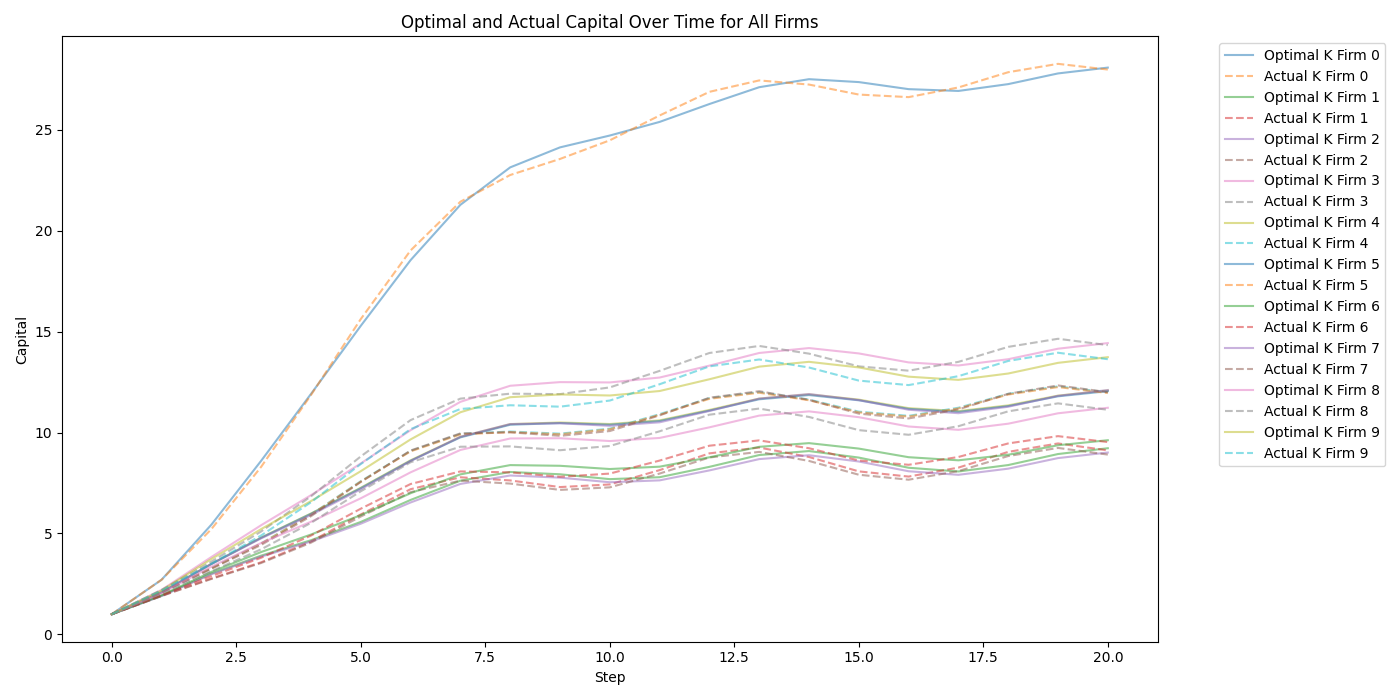
\includegraphics[scale=0.4]{figure/OptimalK_noexit.png}
    \caption{Illustrating a 20-step simulation of 10 firms, this plot compares the chosen optimal capital (\(k\))
    against the
     actual capital (\(k\)) post-business cycle adjustment.}
    \label{fig:optKnoE}
\end{figure}

Following this, the distribution of dividends, based on actual capital, is visualized:
\begin{figure}[H]
    \centering
    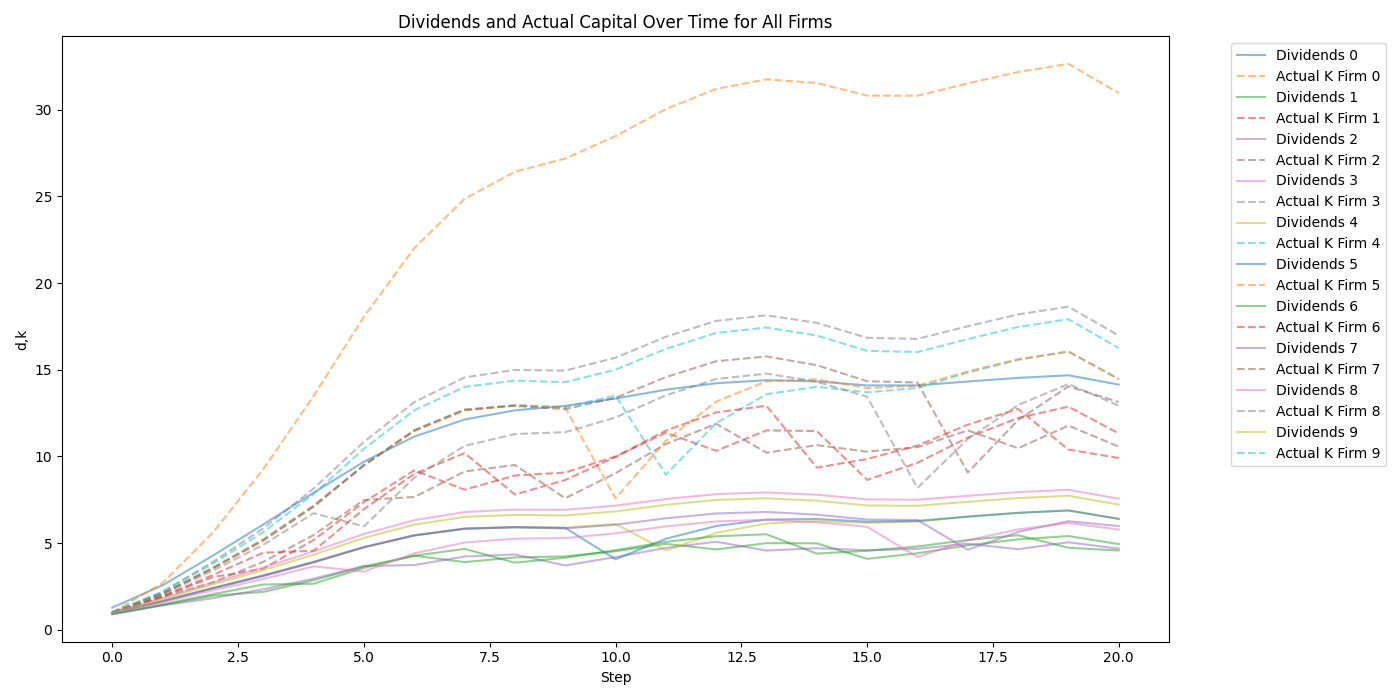
\includegraphics[scale=0.4]{figure/div_cap_noexit.png}
    \caption{Displaying a 20-step simulation for 10 firms, this plot highlights dividends (\( d \)) and the actual capital
    (\(k\)) after business cycle
     adjustments.}
    \label{fig:divNoExit}
\end{figure}

Figure \ref{fig:divNoExit} distinctly shows that firms with superior productivity yield higher dividends. Moreover, upon
achieving a steady state, both capital and dividends exhibit oscillations around a rising mean. 
\begin{figure}[H]
    \centering
    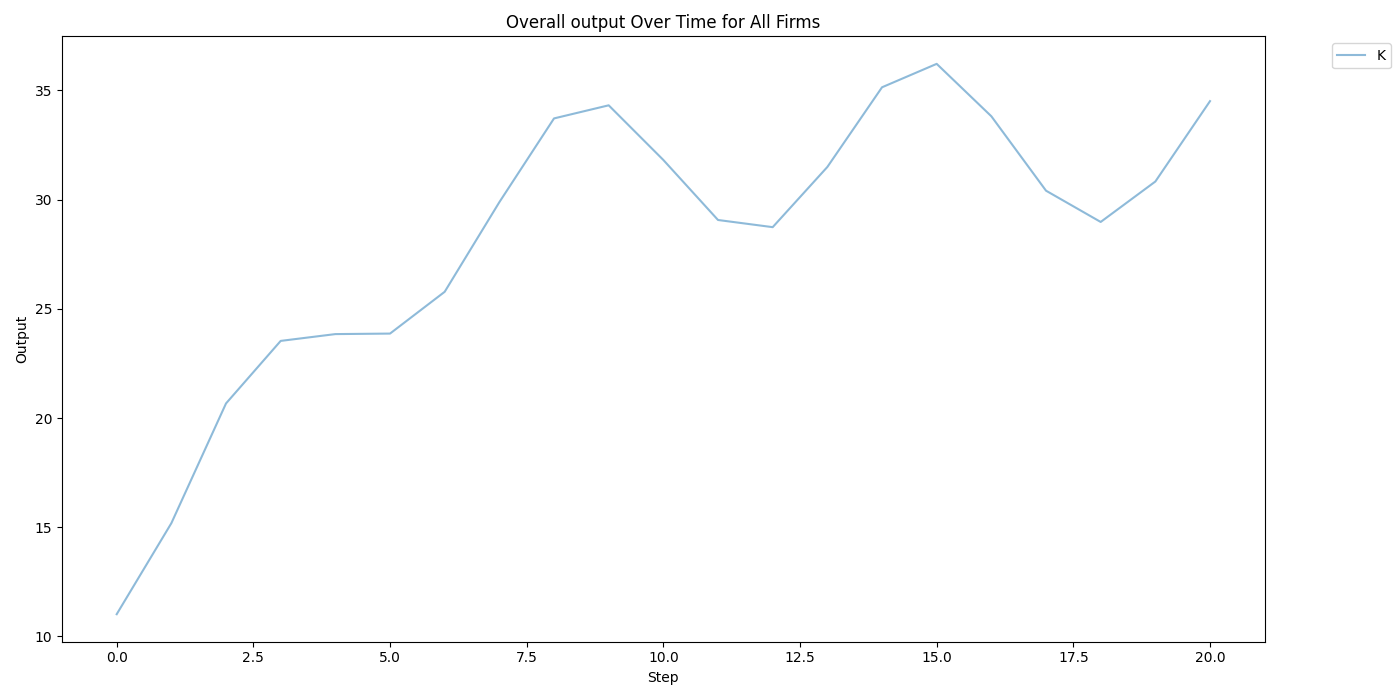
\includegraphics[scale=0.4]{figure/Output_noexit.png}
    \caption{Showcasing a 20-step simulation of 10 firms, this plot reveals the adjusted output (\( K \)) following the business cycle impact.}
    \label{fig:OutNoExit}
\end{figure}


\subsection{The Exit Mechanism}

A firm is prompted to exit the market if its return on capital ranks as the lowest within the firm distribution, making
way for a newcomer who inherits the minimum capital from the existing pool. Subsequently, the exiting firm's capital is
reallocated proportionally among the remaining firms, based on their respective returns on capital. The return on
capital for firm \( i \) at time \( t \) is defined as: 
\[
R_{i,t} = \frac{d_{i,t}}{k_{i,t}}
\]
Should a firm exhibit the \( \min{R} \), it is compelled to exit the market due to possessing the lowest return on capital
among all firms.\footnote{This criterion is enforced at each step, effectively merging the concepts of reallocation and
exit mechanisms henceforth.} 

In the ensuing simulation, while all parameters remain consistent with prior examples, the distinctive feature now is
the market exit of firms. The subsequent figure illustrates both the optimal and actual capital paths for each firm: 

\begin{figure}[H]
    \centering
    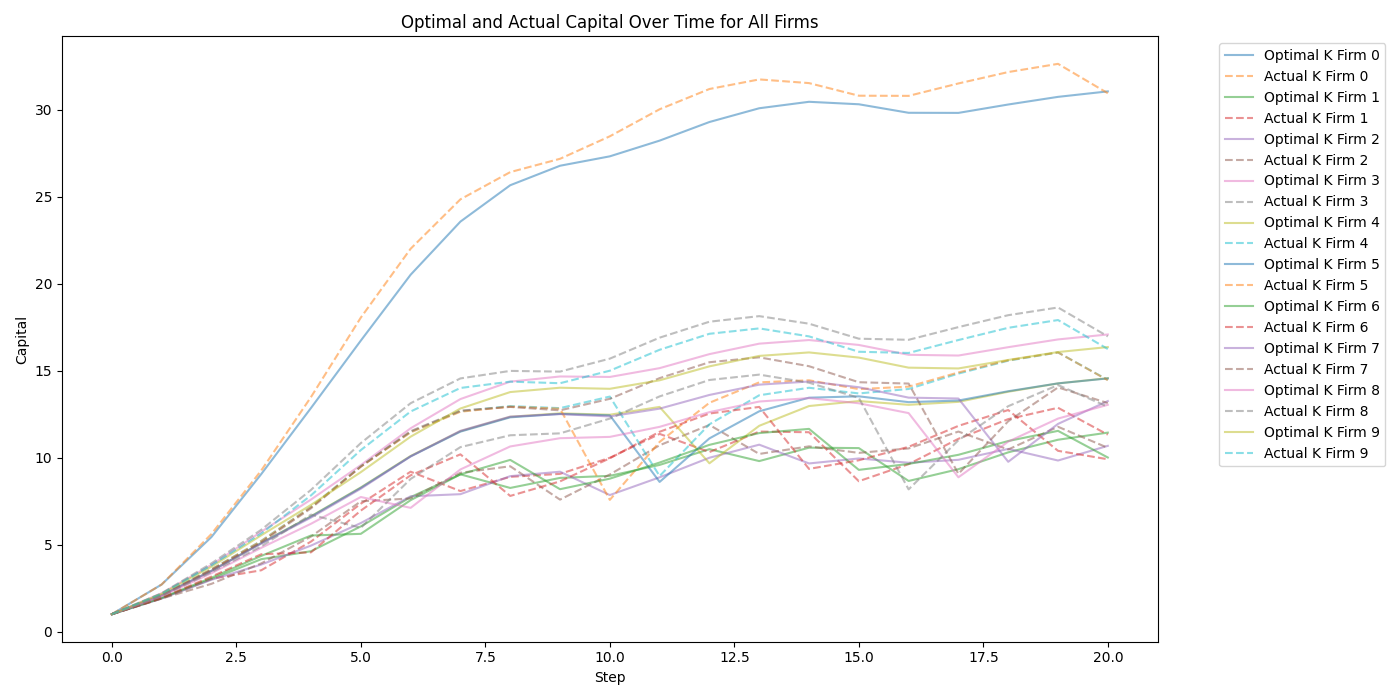
\includegraphics[scale=0.4]{figure/OptimalK_exit.png}
    \caption{Displaying a 20-step simulation involving 10 firms: the optimal \( k \) represents the firm's capital choice,
    whereas the actual \( k \) reflects capital post-adjustment for the business cycle
     effect.}
    \label{fig:optKE}
\end{figure}

Contrasting with previous outcomes, the introduction of an exit mechanism and the redistribution of residual
capital—proportionate to returns, yet ensuring the new entrant retains the minimum capital from the firm
distribution—markedly influences capital trajectory. These mechanisms facilitate incumbent firms in accruing additional
capital, thus hastening their approach to a stationary state, particularly benefiting the most productive entities. This
dynamic underscores the cleansing effect of recessions, as capital reallocation during economic downturns favors
business continuity. The impact of reallocation manifests in the subsequent graph, which delineates a higher
dividends trajectory compared to scenarios devoid of reallocation mechanisms: 

\begin{figure}[H]
    \centering
    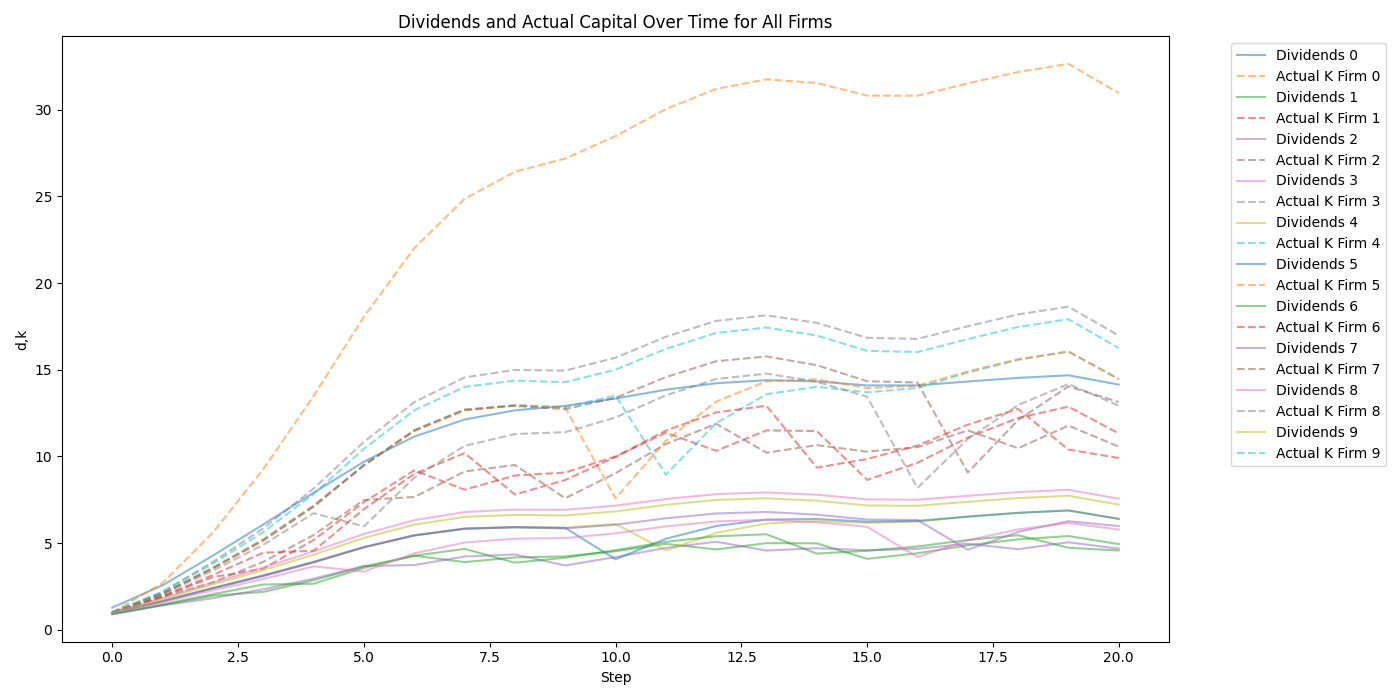
\includegraphics[scale=0.4]{figure/div_cap_exit.png}
    \caption{This figure showcases the results of a 20-step simulation with 10 firms, highlighting dividends (\( d \))
    and actual 
    capital (\( k \)) following business cycle adjustments.}
    \label{fig:divExit}
\end{figure}

Ultimately, examining overall production reveals an uptick attributable to capital reallocation when juxtaposed with
prior simulations, underscoring the efficiency of the exit and reallocation strategies in fostering economic resilience
and growth.


\begin{figure}[H]
    \centering
    \begin{tikzpicture}
    \begin{axis}[
        title={Path of Overall Output},
        xlabel={Time},
        ylabel={\( K \)},
        grid=both,
        minor tick num=1,
        major grid style={lightgray},
        minor grid style={lightgray!25},
        width=0.8\textwidth,
        height=6cm,
    ]
    \addplot[blue] table [col sep=comma, x=Step, y=Total Production] {output_data/exit_nofrictions.csv}; % Blue line for exit mechanism
    \addplot[red] table [col sep=comma, x=Step, y=Total Production] {output_data/noexit_nofrictions.csv}; % Red line for no exit mechanism
    \legend{With Exit Mechanism, Without Exit Mechanism}
    \end{axis}
    \end{tikzpicture}
    \caption{This plot illustrates a 20-step simulation involving 10 firms and demonstrates the impact of the business cycle
    adjustments on overall output \( K \). The blue line represents the scenario incorporating an exit mechanism, whereas
    the red line denotes the scenario without an exit mechanism, illustrating the variations in output across both
     contexts.}
    \label{fig:OutExit}
\end{figure}

Integrating the exit and reallocation mechanisms notably enhances both the dividends' trajectory and the aggregate
output, distinctly highlighting how the cleansing effect bolsters productivity. 


\subsection{Incorporating Financial Frictions into the Model}


In keeping with the methodology set forth in \cite{OsePap17}, financial frictions are incorporated into the model,
parameterized as  \(1-\mu = 0.25\). To discern the cleansing effect amidst financial frictions, an initial simulation is
run where capital remains static due to the absence of a reallocation or exit mechanism. Subsequently, a contrasting
simulation is performed where capital reallocation is possible, with both iterations subjected to financial frictions.

The following plot illustrates the progression of total output over time, displaying two distinct scenarios. The red
line delineates the case without financial frictions, and the blue line portrays the scenario with frictions in place.

\begin{figure}[H]
    \centering
    \begin{tikzpicture}
    \begin{axis}[
        title={Path of Overall Output},
        xlabel={Time},
        ylabel={K},
        grid=both,
        minor tick num=1,
        major grid style={lightgray},
        minor grid style={lightgray!25},
        width=0.8\textwidth,
        height=6cm,
        legend entries={No exit, Exit},
        legend style={at={(0.5,-0.2)},anchor=north,legend cell align=left}
    ]
    \addplot[red, mark=square*] table [col sep=comma, x=Step, y=Total Production] {output_data/noexit_frictions.csv};
    \addplot[blue, mark=otimes*] table [col sep=comma, x=Step, y=Total Production] {output_data/exit_frictions.csv};
    \end{axis}
    \end{tikzpicture}
    \caption{Evolution of the overall output over time. The red line represents the scenario without reallocation and
    exit mechanisms, 
     while the blue line represents the scenario with these mechanisms under financial frictions.}
    \label{fig:output_evolution_frictions}
\end{figure}

Observations indicate that financial frictions attenuate overall production, akin to an effective reduction in
productivity when firms operate with leverage. Although the cleansing effect is evident without financial frictions, it
is imperative to examine whether this effect is sustained when frictions are introduced. To this end, the subsequent plot
juxtaposes the overall output for two comparable financial friction scenarios: one with capital reallocation and one
without.

\begin{figure}[H]
    \centering
    \begin{tikzpicture}
    \begin{axis}[
        title={Path of Overall Output with Financial Frictions},
        xlabel={Time},
        ylabel={K},
        grid=both,
        minor tick num=1,
        major grid style={lightgray},
        minor grid style={lightgray!25},
        width=0.8\textwidth,
        height=6cm,
        legend entries={Reallocation Allowed,No Reallocation},
        legend style={at={(0.5,-0.2)},anchor=north,legend cell align=left}
    ]
    \addplot[blue, mark=*] table [col sep=comma, x=Step, y=Total Production] {output_data/exit_frictions.csv};
    \addplot[red, mark=x] table [col sep=comma, x=Step, y=Total Production] {output_data/noexit_frictions.csv};
    \end{axis}
    \end{tikzpicture}
    \caption{Comparison of overall output with financial frictions over time. The blue line illustrates the output when
    reallocation  
    is allowed, while the red line indicates the output when it is not.}
    \label{fig:output_comparison_frictions}
\end{figure}
Figure \ref{fig:output_comparison_frictions} demonstrates that, even under financial frictions where \(1- \mu =0.25\),
there is a productivity-enhancing mechanism facilitated by capital reallocation due to firm exits. This occurs despite
the presence of asymmetric information between financial intermediaries and firms, as discussed in \cite{OsePap17}.
Furthermore, the cleansing effect on overall production appears to be cumulative, with its impact amplifying over time,
as evidenced by the trend in the graph. Thus, it can be concluded that two economies, identical in their distribution of
productivity and capital among firms and initialized with the same seed\footnote{All simulations were conducted with the
same seed for consistency.}, will diverge in terms of output and productivity if one allows for capital reallocation
through firm exits. This divergence is not only distinct but also grows as time progresses. 
\medskip
\bibliography{reference}

\end{document}











